%% bare_conf_compsoc.tex
%% V1.4b
%% 2015/08/26
%% by Michael Shell
%% See:
%% http://www.michaelshell.org/
%% for current contact information.
%%
%% This is a skeleton file demonstrating the use of IEEEtran.cls
%% (requires IEEEtran.cls version 1.8b or later) with an IEEE Computer
%% Society conference paper.
%%
%% Support sites:
%% http://www.michaelshell.org/tex/ieeetran/
%% http://www.ctan.org/pkg/ieeetran
%% and
%% http://www.ieee.org/

\documentclass[conference,compsoc]{IEEEtran}
% Some/most Computer Society conferences require the compsoc mode option,
% but others may want the standard conference format.
%
% If IEEEtran.cls has not been installed into the LaTeX system files,
% manually specify the path to it like:
% \documentclass[conference,compsoc]{../sty/IEEEtran}

% *** MISC UTILITY PACKAGES ***
%
\usepackage{ifpdf}
\usepackage{framed}
% Heiko Oberdiek's ifpdf.sty is very useful if you need conditional
% compilation based on whether the output is pdf or dvi.
% usage:
% \ifpdf
%   % pdf code
% \else
%   % dvi code
% \fi
% The latest version of ifpdf.sty can be obtained from:
% http://www.ctan.org/pkg/ifpdf
% Also, note that IEEEtran.cls V1.7 and later provides a builtin
% \ifCLASSINFOpdf conditional that works the same way.
% When switching from latex to pdflatex and vice-versa, the compiler may
% have to be run twice to clear warning/error messages.



% *** CITATION PACKAGES ***
%
\ifCLASSOPTIONcompsoc
  % IEEE Computer Society needs nocompress option
  % requires cite.sty v4.0 or later (November 2003)
  \usepackage[nocompress]{cite}
\else
  % normal IEEE
  \usepackage{cite}
\fi



% *** GRAPHICS RELATED PACKAGES ***
%
\ifCLASSINFOpdf
  % \usepackage[pdftex]{graphicx}
  % declare the path(s) where your graphic files are
  % \graphicspath{{../pdf/}{../jpeg/}}
  % and their extensions so you won't have to specify these with
  % every instance of \includegraphics
  % \DeclareGraphicsExtensions{.pdf,.jpeg,.png}
\else
  % or other class option (dvipsone, dvipdf, if not using dvips). graphicx
  % will default to the driver specified in the system graphics.cfg if no
  % driver is specified.
  % \usepackage[dvips]{graphicx}
  % declare the path(s) where your graphic files are
  % \graphicspath{{../eps/}}
  % and their extensions so you won't have to specify these with
  % every instance of \includegraphics
  % \DeclareGraphicsExtensions{.eps}
\fi
% graphicx was written by David Carlisle and Sebastian Rahtz. It is
% required if you want graphics, photos, etc. graphicx.sty is already
% installed on most LaTeX systems. The latest version and documentation
% can be obtained at: 
% http://www.ctan.org/pkg/graphicx
% Another good source of documentation is "Using Imported Graphics in
% LaTeX2e" by Keith Reckdahl which can be found at:
% http://www.ctan.org/pkg/epslatex
%
% latex, and pdflatex in dvi mode, support graphics in encapsulated
% postscript (.eps) format. pdflatex in pdf mode supports graphics
% in .pdf, .jpeg, .png and .mps (metapost) formats. Users should ensure
% that all non-photo figures use a vector format (.eps, .pdf, .mps) and
% not a bitmapped formats (.jpeg, .png). The IEEE frowns on bitmapped formats
% which can result in "jaggedy"/blurry rendering of lines and letters as
% well as large increases in file sizes.
%
% You can find documentation about the pdfTeX application at:
% http://www.tug.org/applications/pdftex





% *** MATH PACKAGES ***
%
\usepackage{amsmath}
\usepackage{cuted}
% A popular package from the American Mathematical Society that provides
% many useful and powerful commands for dealing with mathematics.
%
% Note that the amsmath package sets \interdisplaylinepenalty to 10000
% thus preventing page breaks from occurring within multiline equations. Use:
%\interdisplaylinepenalty=2500
% after loading amsmath to restore such page breaks as IEEEtran.cls normally
% does. amsmath.sty is already installed on most LaTeX systems. The latest
% version and documentation can be obtained at:
% http://www.ctan.org/pkg/amsmath
\newcommand\numberthis{\addtocounter{equation}{1}\tag{\theequation}}




% *** SPECIALIZED LIST PACKAGES ***
%
\usepackage{algorithmic}
% algorithmic.sty was written by Peter Williams and Rogerio Brito.
% This package provides an algorithmic environment fo describing algorithms.
% You can use the algorithmic environment in-text or within a figure
% environment to provide for a floating algorithm. Do NOT use the algorithm
% floating environment provided by algorithm.sty (by the same authors) or
% algorithm2e.sty (by Christophe Fiorio) as the IEEE does not use dedicated
% algorithm float types and packages that provide these will not provide
% correct IEEE style captions. The latest version and documentation of
% algorithmic.sty can be obtained at:
% http://www.ctan.org/pkg/algorithms
% Also of interest may be the (relatively newer and more customizable)
% algorithmicx.sty package by Szasz Janos:
% http://www.ctan.org/pkg/algorithmicx




% *** ALIGNMENT PACKAGES ***
%
\usepackage{array}
% Frank Mittelbach's and David Carlisle's array.sty patches and improves
% the standard LaTeX2e array and tabular environments to provide better
% appearance and additional user controls. As the default LaTeX2e table
% generation code is lacking to the point of almost being broken with
% respect to the quality of the end results, all users are strongly
% advised to use an enhanced (at the very least that provided by array.sty)
% set of table tools. array.sty is already installed on most systems. The
% latest version and documentation can be obtained at:
% http://www.ctan.org/pkg/array


% IEEEtran contains the IEEEeqnarray family of commands that can be used to
% generate multiline equations as well as matrices, tables, etc., of high
% quality.




% *** SUBFIGURE PACKAGES ***
%\ifCLASSOPTIONcompsoc
%  \usepackage[caption=false,font=footnotesize,labelfont=sf,textfont=sf]{subfig}
%\else
%  \usepackage[caption=false,font=footnotesize]{subfig}
%\fi
% subfig.sty, written by Steven Douglas Cochran, is the modern replacement
% for subfigure.sty, the latter of which is no longer maintained and is
% incompatible with some LaTeX packages including fixltx2e. However,
% subfig.sty requires and automatically loads Axel Sommerfeldt's caption.sty
% which will override IEEEtran.cls' handling of captions and this will result
% in non-IEEE style figure/table captions. To prevent this problem, be sure
% and invoke subfig.sty's "caption=false" package option (available since
% subfig.sty version 1.3, 2005/06/28) as this is will preserve IEEEtran.cls
% handling of captions.
% Note that the Computer Society format requires a sans serif font rather
% than the serif font used in traditional IEEE formatting and thus the need
% to invoke different subfig.sty package options depending on whether
% compsoc mode has been enabled.
%
% The latest version and documentation of subfig.sty can be obtained at:
% http://www.ctan.org/pkg/subfig
\usepackage{verbatim}
\usepackage{soul}
\usepackage{xcolor}
\newcommand{\TODO}[1]{\hl{TODO: #1}}
\newcommand{\NOTE}[1]{\hl {NOTE: #1}}
\newcommand{\changed}[1]{\textcolor{red}{#1}}


% *** FLOAT PACKAGES ***
%
%\usepackage{fixltx2e}
% fixltx2e, the successor to the earlier fix2col.sty, was written by
% Frank Mittelbach and David Carlisle. This package corrects a few problems
% in the LaTeX2e kernel, the most notable of which is that in current
% LaTeX2e releases, the ordering of single and double column floats is not
% guaranteed to be preserved. Thus, an unpatched LaTeX2e can allow a
% single column figure to be placed prior to an earlier double column
% figure.
% Be aware that LaTeX2e kernels dated 2015 and later have fixltx2e.sty's
% corrections already built into the system in which case a warning will
% be issued if an attempt is made to load fixltx2e.sty as it is no longer
% needed.
% The latest version and documentation can be found at:
% http://www.ctan.org/pkg/fixltx2e


%\usepackage{stfloats}
% stfloats.sty was written by Sigitas Tolusis. This package gives LaTeX2e
% the ability to do double column floats at the bottom of the page as well
% as the top. (e.g., "\begin{figure*}[!b]" is not normally possible in
% LaTeX2e). It also provides a command:
%\fnbelowfloat
% to enable the placement of footnotes below bottom floats (the standard
% LaTeX2e kernel puts them above bottom floats). This is an invasive package
% which rewrites many portions of the LaTeX2e float routines. It may not work
% with other packages that modify the LaTeX2e float routines. The latest
% version and documentation can be obtained at:
% http://www.ctan.org/pkg/stfloats
% Do not use the stfloats baselinefloat ability as the IEEE does not allow
% \baselineskip to stretch. Authors submitting work to the IEEE should note
% that the IEEE rarely uses double column equations and that authors should try
% to avoid such use. Do not be tempted to use the cuted.sty or midfloat.sty
% packages (also by Sigitas Tolusis) as the IEEE does not format its papers in
% such ways.
% Do not attempt to use stfloats with fixltx2e as they are incompatible.
% Instead, use Morten Hogholm'a dblfloatfix which combines the features
% of both fixltx2e and stfloats:
%
% \usepackage{dblfloatfix}
% The latest version can be found at:
% http://www.ctan.org/pkg/dblfloatfix




% *** PDF, URL AND HYPERLINK PACKAGES ***
%
\usepackage{url}
% url.sty was written by Donald Arseneau. It provides better support for
% handling and breaking URLs. url.sty is already installed on most LaTeX
% systems. The latest version and documentation can be obtained at:
% http://www.ctan.org/pkg/url
% Basically, \url{my_url_here}.

\usepackage{graphicx} % Required for including pictures
\graphicspath{{pics/}} % Specifies the directory where pictures are stored
\usepackage{caption}
\usepackage{subcaption}
\usepackage{booktabs}
\usepackage{multirow} % make table

\makeatletter % Put Roman Number in Text
\newcommand{\rmnum}[1]{\romannumeral #1}
\newcommand{\Rmnum}[1]{\expandafter\@slowromancap\romannumeral #1@}
\makeatother



% *** Do not adjust lengths that control margins, column widths, etc. ***
% *** Do not use packages that alter fonts (such as pslatex).         ***
% There should be no need to do such things with IEEEtran.cls V1.6 and later.
% (Unless specifically asked to do so by the journal or conference you plan
% to submit to, of course. )


% correct bad hyphenation here
\hyphenation{op-tical net-works semi-conduc-tor}


\begin{document}
%
% paper title
% Titles are generally capitalized except for words such as a, an, and, as,
% at, but, by, for, in, nor, of, on, or, the, to and up, which are usually
% not capitalized unless they are the first or last word of the title.
% Linebreaks \\ can be used within to get better formatting as desired.
% Do not put math or special symbols in the title.
\title{Watch Out for the Bully! Job Interference Study on Dragonfly Network}


% author names and affiliations
% use a multiple column layout for up to three different
% affiliations
% \author{\IEEEauthorblockN{Michael Shell}
% \IEEEauthorblockA{School of Electrical and\\Computer Engineering\\
% Georgia Institute of Technology\\
% Atlanta, Georgia 30332--0250\\
% Email: http://www.michaelshell.org/contact.html}
% \and
% \IEEEauthorblockN{Homer Simpson}
% \IEEEauthorblockA{Twentieth Century Fox\\
% Springfield, USA\\
% Email: homer@thesimpsons.com}
% \and
% \IEEEauthorblockN{James Kirk\\ and Montgomery Scott}
% \IEEEauthorblockA{Starfleet Academy\\
% San Francisco, California 96678-2391\\
% Telephone: (800) 555--1212\\
% Fax: (888) 555--1212}}


\author{

\IEEEauthorblockN{Xu Yang\IEEEauthorrefmark{1}, John Jenkins\IEEEauthorrefmark{2}, Misbah Mubarak\IEEEauthorrefmark{2}, Robert B. Ross\IEEEauthorrefmark{2}, Zhiling Lan\IEEEauthorrefmark{1}}

\IEEEauthorblockA{\IEEEauthorrefmark{1}Department of Computer Science,
Illinois Institute of Technology,
Chicago, Illinois, USA 60616\\
\{xyang56\}@hawk.iit.edu, lan@iit.edu}

\IEEEauthorblockA{\IEEEauthorrefmark{2}Mathematics and Computer Science Division, Argonne National Laboratory,
Argonne, IL, USA 60439\\
\{jenkins,rross\}@mcs.anl.gov, mmubarak@anl.gov}
}


% conference papers do not typically use \thanks and this command
% is locked out in conference mode. If really needed, such as for
% the acknowledgment of grants, issue a \IEEEoverridecommandlockouts
% after \documentclass

% for over three affiliations, or if they all won't fit within the width
% of the page (and note that there is less available width in this regard for
% compsoc conferences compared to traditional conferences), use this
% alternative format:
% 
%\author{\IEEEauthorblockN{Michael Shell\IEEEauthorrefmark{1},
%Homer Simpson\IEEEauthorrefmark{2},
%James Kirk\IEEEauthorrefmark{3}, 
%Montgomery Scott\IEEEauthorrefmark{3} and
%Eldon Tyrell\IEEEauthorrefmark{4}}
%\IEEEauthorblockA{\IEEEauthorrefmark{1}School of Electrical and Computer Engineering\\
%Georgia Institute of Technology,
%Atlanta, Georgia 30332--0250\\ Email: see http://www.michaelshell.org/contact.html}
%\IEEEauthorblockA{\IEEEauthorrefmark{2}Twentieth Century Fox, Springfield, USA\\
%Email: homer@thesimpsons.com}
%\IEEEauthorblockA{\IEEEauthorrefmark{3}Starfleet Academy, San Francisco, California 96678-2391\\
%Telephone: (800) 555--1212, Fax: (888) 555--1212}
%\IEEEauthorblockA{\IEEEauthorrefmark{4}Tyrell Inc., 123 Replicant Street, Los Angeles, California 90210--4321}}




% use for special paper notices
%\IEEEspecialpapernotice{(Invited Paper)}




% make the title area
\maketitle

% As a general rule, do not put math, special symbols or citations
% in the abstract
\begin{abstract}

The high-radix, low-diameter dragonfly network will be the choice of many computing facilities for building their next generation supercomputers. 
Preliminary studies show that random placement with adaptive routing should be the rule of thumb to utilize such networks for it can uniformly distribute traffic and alleviate congestion. 
However, in this paper, we made the observation that while random placement coupled with adaptive routing can load-balance the network, it can not guarantee the best performance for every single job.
The performance improvement of communication-intensive jobs comes with at the cost of performance degradation of less intensive jobs. 
We identify this ``bully" behavior and validate its underneath causes with the help of detailed network simulation and real application traces.
We propose a hybrid job placement policy providing either contiguous or random allocation to each application based on its communication intensity. 
Our experiment results demonstrate that this hybrid job placement policy can lead to performance improvement for less communication-intensive applications.


%We refer this phenomenon as ``bully" between concurrently running jobs. We presented a detailed analysis about this ``bully" behavior between jobs at the network level based on a sophisticated, high-fidelity discrete even-driven simulation tool. The observations and analysis presented in this work illuminate a path to the adoption of more efficient job placement policy and routing algorithm for HPC systems with dragonfly network.  

\end{abstract}

% no keywords

% \keywords{Dragonfly, Job placement, Routing, Interference}



% For peer review papers, you can put extra information on the cover
% page as needed:
% \ifCLASSOPTIONpeerreview
% \begin{center} \bfseries EDICS Category: 3-BBND \end{center}
% \fi
%
% For peerreview papers, this IEEEtran command inserts a page break and
% creates the second title. It will be ignored for other modes.
\IEEEpeerreviewmaketitle


\section{Introduction}
\label{sec:intro}

Low-latency and high-bandwidth interconnect networks play a critical role in ensuring HPC system performance. 
The high-radix, low-diameter dragonfly topology can lower the overall cost of the interconnect, improve network bandwidth and reduce packet latency \cite{dally-dragonfly}, 
making it a very promising choice for building supercomputers with millions of cores.
Even with such powerful networks, 
intelligent job placement is of paramount importance to the efficient use of dragonfly connected systems~\cite{bhatele2015, jain-sc14}. 
%An ideal job placement policy should not only load balance the network 
%but also guarantee the performance of every single application by minimizing the inevitable interference on the dragonfly network.  

Recent studies suggest that random node allocation for parallel jobs, coupled
with adaptive routing, can alleviate local congestion, eliminate hot-spots and achieve load-balancing for dragonfly networks~\cite{jain-sc14, bhatele-sc11, brandt2014}. 
These works explore the possible job placement and routing configurations that could optimize the overall network performance without examining how different configurations impact the progress of individual applications.
In this paper, we study the implications of contention for shared network links in the context of multiple HPC applications running on dragonfly systems when different job placement and routing configurations are in use.
Our analyses focus on the overall network performance as well as the performance of concurrently executing applications in the presence of network contention.

%We have observed that when running concurrently on the dragonfly network, applications interfere with each other and the less communication-intensive applications are ``bullied" by the communication-intensive ones. The ``bully" applications get great performance improvement at the cost of performance degradation to the ``bullied" applications. We choose three representative applications from the DOE Design Forward Project~\cite{designforwardwebpage} to study the root cause of the ``bullying" with simulation on CODES, an high-fidelity, packet-level HPC network simulation toolkit~\cite{codes}. 


We choose three representative HPC applications from the DOE Design Forward Project~\cite{designforward-webpage} and analyze the interference among them. Our study is based on simulation with CODES, a high-fidelity, flit-level HPC network simulation toolkit~\cite{misbah-tpds}. 
For each application, we examine its performance with two job placement policies and three routing policies.
We make the following observations through extensive simulations.


%In this work, we study the interference between concurrently running jobs on dragonfly networks with different job placement and routing policies. We use CODES, an HPC network simulation toolkit with high fidelity and excellent scalability for packet level simulation \cite{codes}. Unlike much existing work that rely on synthetic workloads, we use traces of three representative applications from the DOE Design Forward Project \cite{designforwardwebpage}. The advantage of using real application traces is straight forward: these traces can capture detailed application communication behaviors that are omitted in synthetic workload for simplification. Applications are usually distinctive from each other in data transfer amount, communication pattern, operation dependency etc., which can be impractical to reproduce in a synthetic workload.

%We conduct extensive experiments with three applications running on dragonfly network with two job placement policies and three routing policies. We analyze the performance of network as well as individual application when running with different placement and routing configurations. Our evaluation is based on more than 1000 runs of simulation. We make the following interesting observations through extensive simulation.


\begin{itemize}
   
    \item Concurrently running applications on a dragonfly network interfere with each other when they share network resources. Communication-intensive applications ``bully" their less intensive peers and obtain performance improvement at the expense of less intensive ones. 
    
    \item Random placement of application processes in the dragonfly can improve the performance of communication-intensive applications by enabling network resource sharing, though it introduces interference causing performance degradation to the less intensive applications.
    
   \item Contiguous placement can be beneficial to the consistent performance of less communication-intensive applications by minimizing network resource sharing, because it reduces the opportunities for traffic from other applications to be loaded on links that serve as minimal routes for the less intensive application. However, this comes with the downside of at times greatly reduced system performance via load imbalance.
    
    
\end{itemize}

Based on the aforementioned key observations, one would expect that an ideal job placement policy on dragonfly systems would take relative communication intensity into account, and mix contiguous and non-contiguous placement based on application needs. To explore this expectation, we investigate a hybrid job placement policy, which assigns random allocations to communication-intensive applications and contiguous allocations to less intensive ones. Initial experimentation shows that hybrid job placement aids in reducing the worst-case performance degradation for less communication-intensive applications while retaining the performance of communication-intensive applications, though without eliminating the problem entirely.
%\emph{The random placement and adaptive routing are preferable to communication-intensive jobs, whereas contiguous placement and minimal routing are in favor of less intensive jobs.} 
To the best of our knowledge, using real application traces from production systems for the study of job interference on dragonfly networks has not been reported in the literature so far. We believe the observations and new placement policy presented in this paper are valuable to the HPC community.
%We believe the observations and new placement policy presented in this paper are valuable to a number of communities including HPC computing centers, system software developers, and system administrators. 
%For example, the computing centers should take resource sharing into consideration when choosing proper configurations for building their dragonfly networks. System software developers could design better scheduling algorithms for jobs with distinct communication behavior. System administrators could make more accurate predication about system availability based on job running status under different placement and routing configurations.


The rest of this paper is organized as follows. Section~\ref{sec:background} describes an implementation of the dragonfly network, introduces the placement policies and routing policies. Section~\ref{sec: methodology} talks about the use of CODES as a research vehicle and three representative applications from the DOE Design Forward Project. Section~\ref{sec:workload-1} presents the observations and analysis of three applications running on a dragonfly network with different placement and routing configurations. Section~\ref{sec:workload-2} validates the observations we obtain from previous section. Section~\ref{sec: hybrid placement} presents a alternative placement policy for the dragonfly network. Section~\ref{sec:related work} discusses the related work. Finally, the conclusion is presented in Section~\ref{sec:conclusion}.





\section{Background}
\label{sec:background}

In this section, we review the dragonfly topology, including the placement and routing policies examined in previous work. 

\subsection{Dragonfly Network}
\label{sec:network}
The dragonfly is a two-level hierarchical topology, consisting of several groups connected by all-to-all links. In each group, there could be $a$ routers connected via all-to-all local channels. For each router, there could be $p$ compute nodes attached to it via terminal links. The router has $h$ global channels used as intergroup connections through which it connected to other routers in different groups. Thus, the radix of each router is $k = a+h+p-1$. Different computing centers could choose different values for  $a$, $h$, $p$ when deploying their dragonfly network. The adoption of proper $a$, $h$, $p$ involves many factors such as system scale, building cost and workload characteristics. 

It is recommended that for the load balance purpose, a proper dragonfly configuration should follow $a=2p=2h$~\cite{kim-micro}. According to this configuration, the total number of groups, denoted as $g$ in the dragonfly network would be $g = a*h+1 $, the total number of compute nodes denoted as $N$ in the network would be $N = p*a*g $. An implementation of dragonfly network follows such configuration is illustrated in Figure~\ref{fig:dragonfly-overview}. There are six routers in each group, each router has three compute nodes attached to it. This dragonfly network consists of 19 groups and 342 nodes in total.

\begin{figure}[h!] 
  \centering
  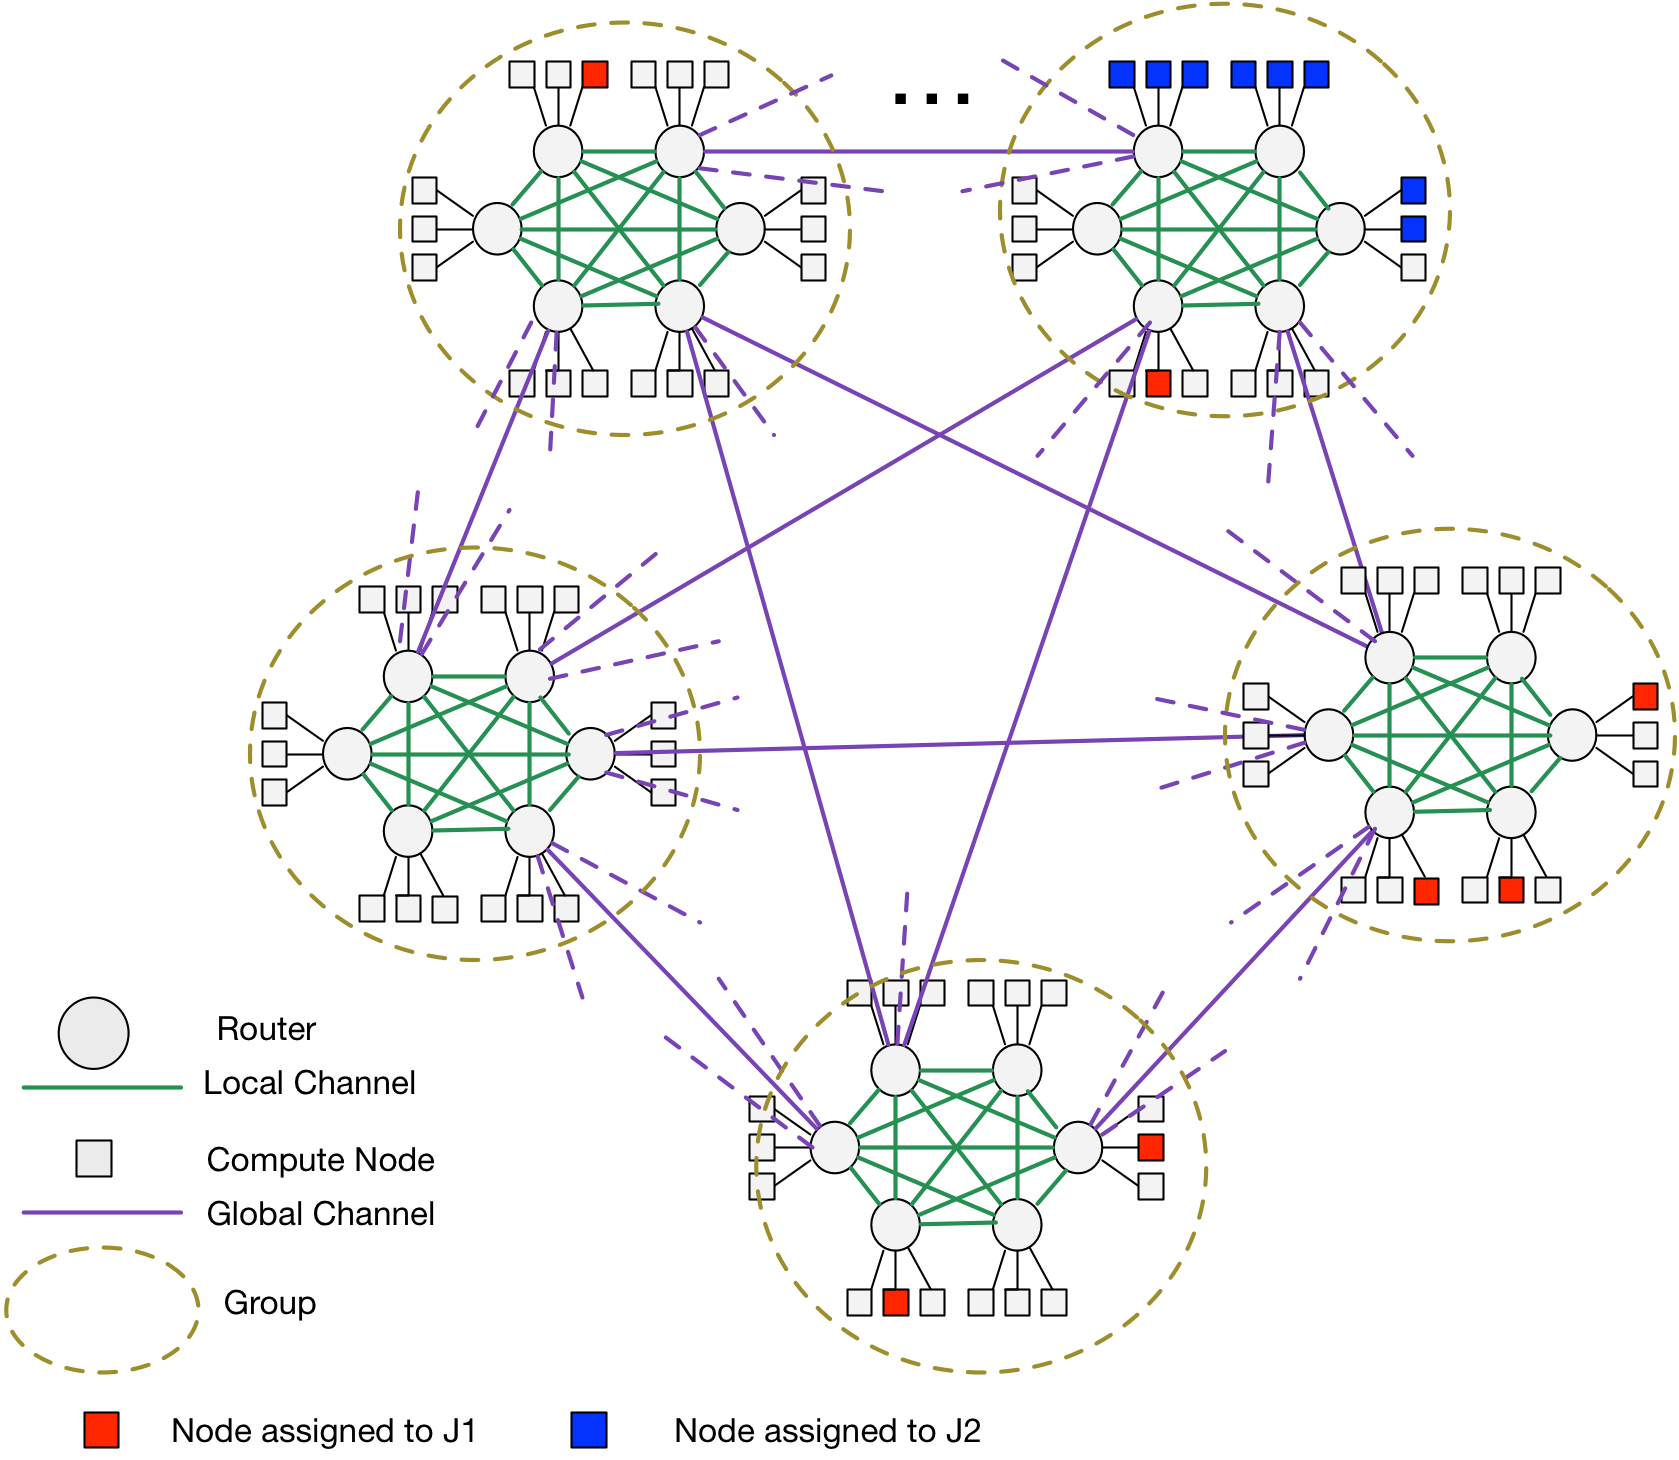
\includegraphics[width=0.48\textwidth]{dragonfly-overview}
  \caption{Dragonfly Network Overview. There are 19 groups, six routers in each group, three compute nodes connected to each router, 342 nodes in total. Job $J1$ requires seven nodes, getting its allocation by random placement. Job $J2$ requires eight nodes, getting its allocation by contiguous placement.}
  \label{fig:dragonfly-overview}
\end{figure}


\subsection{Job Placement on Dragonfly}
\label{sec:placement-schemes}

For a parallel application requiring multiple compute nodes, job placement policy refers to the way of assigning the required number of nodes to the application by a system software such as batch scheduler~\cite{xu-cluster14}. In this work, we study two alternative placement policies considered by the community for dragonfly systems: 

\textbf{Random Placement:} In this policy, an application gets the required number of nodes randomly selected from all the available nodes in the system. As illustrated in Figure~\ref{fig:dragonfly-overview}, $J1$ gets random allocation in which nodes are attached to different routers in different groups. Routers may be shared by different applications and more routers are involved in serving each application when random placement is in use. Random placement can distribute the tasks of an application uniformly across the network to avoid the possible local congestion. However, random placement may cause congestion on global links.


\textbf{Contiguous Placement:} In this policy, the compute nodes are assigned to an application in a consecutive manner. The assignment first fills up a group, then crosses group boundaries and starts to fill the next group if necessary. As illustrated in Figure~\ref{fig:dragonfly-overview}, $J2$ gets eight nodes by contiguous placement. Contiguous placement confines the tasks of an application into the same group and uses minimum number of routers serving each application, which may result in local network congestion and increase the possibility of hot-spots. 


\subsection{Routing on Dragonfly}
\label{sec:routing-schemes}

The routing policy refers to the strategy adopted to route a message (a stream of packets) from the source router to the destination router. Previously studied routing policies for dragonfly network include minimal routing, adaptive routing~\cite{dally-dragonfly}, progressive adaptive routing~\cite{jiang} and some of their variations~\cite{won-prog-adaptive}. In this work we study three alternative routing policies considered by the community for dragonfly networks.

\textbf{Minimal:} In this policy, a message takes the shortest path from the source router to the destination router. When there are multiple shortest paths between the source and destination, the message will be evenly divided among the paths. Minimal routing can guarantee the minimum hops the message takes from the source to the destination. However, it may result in congestion along the shortest paths. 

\textbf{Adaptive:} In this policy, the path a message takes will be adaptively chosen between shortest and non-shortest paths, depending on the congestion situation along those paths. For the non-shortest path, an intermediate router will be randomly chosen. The message takes the intermediate router as a via point, connecting the source and destination router through two separate shortest paths. Adaptive routing can avoid hot-spots in the presence of congestion and collapse to minimal routing otherwise. 

\textbf{Progressive Adaptive:} In this policy, the decision to route minimally at each hop in the source group will be re-evaluated. Any decision to route non-minimally at source router or at a subsequent hop is permanent and will not be re-evaluated~\cite{jiang}. The progressive adaptive is capable of handling the case when a global channel is congested but the source router has not been informed yet~\cite{jiang}. The packet will take the non-minimal route only when the congestion is encountered. 






\section{Methodology}
\label{sec: methodology}

Configurable dragonfly networks that allow us to perform the exploration presented in this paper are hard to come by for the time being. Even with access to systems with such networks, job placement and routing policies are part of system configuration, which is impossible for user to make changes at will~\cite{jain-sc14, bhatele-sc11, zhou-ipdps-2015, jokanovic-ipdps-2015}. Therefore, we resort to simulation in our work.


%It is difficult to experiment with concurrently running jobs on HPC systems~\cite{zhou-ipdps-2015}\cite{jain-sc14}\cite{bhatele-sc11}\cite{jokanovic-ipdps-2015}. One reason is that job placement and routing policies are part of system configuration, which is impossible for user to make changes at will. Another reason is that it is unrealistic to reserve the system exclusively to run the same batch of jobs with desired placement and routing configurations and compare the results. The third reason is that configurable dragonfly networks that allow us to perform the exploration presented in this paper are hard to come by for the time being. Therefore, we resort to simulation in our work.

\subsection{Simulation Tool}
\label{sec:simulation-tool}

We utilize the CODES simulation toolkit (Co-Design of Multilayer Exascale Storage Architectures)~\cite{codes}, which builds upon the ROSS parallel discrete event simulator~\cite{carothers_ross:_2002,barnes_warp_2013} to enable exploratory study of large scale systems of interest to the HPC community. CODES supports dragonfly~\cite{codes-dragonfly, misbah-tpds}, torus~\cite{misbah-pads-2014, ning-pads-2011}, and fat-tree~\cite{ning-pads-2015} networks with flit-level high-fidelity simulation. It can drive these models through an MPI simulation layer utilizing traces generated by the DUMPI MPI tracer~\cite{sst}.

\subsection{Parallel Applications}
\label{sec: application traces}

We use a trace-driven approach to workload generation, choosing in particular three parallel application traces gathered to represent exascale workload behavior as part of the DOE Design Forward Project~\cite{designforwardwebpage} \TODO{can we get a better cite?}. Specifically, we study communication traces representing the \emph{Algebraic MultiGrid Solver} (AMG), \emph{Geometric Multigrid V-Cycle from Production Elliptic Solver} (MultiGrid) and \emph{Crystal Router MiniApp} (CrystalRouter).

\textbf{AMG:} The Algebraic MultiGrid Solver is a parallel algebraic multi-grid solver for linear systems arising from problems on unstructured mesh physics packages. It has been derived directly from the BoomerAMG solver developed in the Center for Applied Scientific Computing (CASC) at LLNL~\cite{amg}. 


\textbf{MultiGrid:} The geometric multi-grid v-cycle from the production elliptic solver BoxLib is a software framework for massively parallel block-structured adaptive mesh refinement (AMR) codes~\cite{boxlib}, which are used in structured grid physics packages. 

\textbf{CrystalRouter:} The Crystal Router MiniApp is a communication kernel of Nek5000~\cite{nek5000}, a spectral element CFD application developed at Argonne National Laboratory. It features spectral element multi-grid solvers coupled with a highly scalable, parallel coarse-grid solver that is widely used for projects including ocean current modeling, thermal hydraulics of reactor cores, and spatiotemporal chaos. 




\subsection{System Configuration}
\label{sec: simulation configuration}

The parameters for building the dragonfly network studied in our work are informed by the model proposed by Kim et al.~\cite{kim-micro}. Our dragonfly network consists of 33 groups, each containing eight routers. Each router has four compute nodes attached to it. Overall, there are 264 routers and 1056 compute nodes in the network. \TODO{What's the resulting router radix? What's the classic $a,h,p$ (or whatever they are :) parameters?} The aggregate bandwidth of the terminal links, as well as the local and global channels, are proportional to those of the Cray Cascade system~\cite{faanes} \TODO{What are these bandwidths?}. In this work, we simulate the network performance and job interference across six different job placement and routing policy combinations, which are summarized in Table~\ref{tab: placement routing configs}.

%\footnote{With respect to random placement, we experiment with 50 sets of distinctive allocation generated by random placement. The corresponding experimental results are median chosen, which intended to eliminate the possibility of variation.}

\begin{table}[ht]
\begin{center}
\caption{The notation for different placement and routing configurations.} 
\label{tab: placement routing configs}
\begin{tabular}{l c c c }
\toprule % Top horizontal line
\toprule
&\multicolumn{3}{c}{Routing Policies} \\ 
\cmidrule(l){2-4}
Placement Policies & Minimal & Adaptive & Progressive Adaptive\\ % Column names row
\midrule % In-table horizontal line
Contiguous  &  CM   &   CA   &  CPA   \\ % Content row 1
\midrule
Random  &   RM  &   RA   &  RPA   \\ 
\midrule % In-table horizontal line
\bottomrule % Bottom horizontal line
\end{tabular}
\end{center}
\end{table}


We analyze both the overall network performance and the performance of every single application.
Our analysis focuses on the following metrics:
\begin{itemize}

    \item \textbf{Network Traffic:} The traffic refers to the amount of data going through each router. We analyze the traffic on the terminal link, local and global channel of each router. The network reaches optimal performance when the traffic is uniformly distributed and no particular router is over-loaded. 
            
    \item \textbf{Network Saturation Time:} The saturation time refers to the time period when the buffer of a certain port in the router is full. We analyze the saturation time of ports corresponding to terminal links, local and global channels. The saturated time indicates the congestion level of routers. 
    
    \item \textbf{Communication Time:} The communication time of each MPI rank refers to the time it spends in completing all its message exchanges with other ranks. Due to our use of simulation, we are able to measure the absolute (simulated) time a message takes to reach its destination. \TODO{Verify this. Or is comm time the time that the terminal link is busy?} The performance of each application is measured by the \TODO{max? avg across ranks? distribution?} communication time.
\end{itemize}

Note that we do not model computation for each MPI rank due to both the complexities inherent in performance prediction on separate parallel architectures as well as the emphasis on the side of the Design Forward traces on communication behavior rather than compute representation; users are instructed to treat the traces as if they came from one MPI rank-per-node configuration, despite being gathered using a rank-per-core approach. We instead allow MPI communications to proceed as quickly as they are able. \TODO{is this a good enough explanation? Anything else we should add?}

\subsection{Workload Summary}
\label{sec:workload summary}

Two sets of parallel workloads are used in this study. Workload~\Rmnum{1} consists of AMG, MultiGrid and CrystalRouter. As shown in Table~\ref{tab:apps-detail}, AMG has the least amount of data transfer, making it the least communication-intensive job in the workload. Workload~\Rmnum{2} consists of sAMG, MultiGrid and CrystalRouter. sAMG, a synthetic version of AMG, is generated by increasing the data transferred in AMG's MPI calls by a factor of 100, making it the most communication-intensive job in the workload. We do this for reasons that will become clear in the following sections.

Each rank of each application is run on a dedicated node, following the recommended interpretation of the traces by the Design Forward team.

%Table \ref{tab:apps-detail} summarizes the details of each application. It shows the number of MPI ranks, the average data transfer amount of each rank and the total data transfer amount for each application.

\begin{table}[ht]
\begin{center}
\caption{Application Summaries}
\label{tab:apps-detail}
\begin{tabular}{l c c c }
\toprule % Top horizontal line
\toprule
App Name & Num. Rank & Avg. Data/Rank & Total Data\\ % Column names row
\midrule % In-table horizontal line
AMG  &    216 &   0.6MB   &     130MB\\ % Content row 1
\midrule
MultiGrid  &    125 &   5MB   &     625MB\\ 
\midrule
CrystalRouter  &   100  &  35MB    &     3500MB\\ 
\midrule
sAMG  &    216 &   60MB   &     13000MB\\ % Content row 1
\midrule % In-table horizontal line
\bottomrule % Bottom horizontal line
\end{tabular}
\end{center}
\end{table}




\section{Study of Parallel Workload~\Rmnum{1}}
%\section{Identify the ``Bully"}
\label{sec:workload-1}

The study of Workload~\Rmnum{1} consists of two parts. First, we analyze the overall network performance when Workload~\Rmnum{1} is running under different placement and routing configurations. Second, we isolate each application from the workload and analyze its performance on both a per-rank basis as well as by considering router traffic resident to application ranks. The analysis allows us to identify the ``bully'' in Workload~\Rmnum{1}.

\TODO{Add in a few words across the section (not here) on how previous work compares as you go through the results.}

\subsection{Network Performance Analysis}
\label{sec: workload-1 network analysis}

We first study the network performance at the system level by analyzing the degree of traffic and saturation seen at each router.

\begin{figure*}[t!]
    \centering
    \begin{subfigure}[t]{0.32\textwidth}
        \centering
        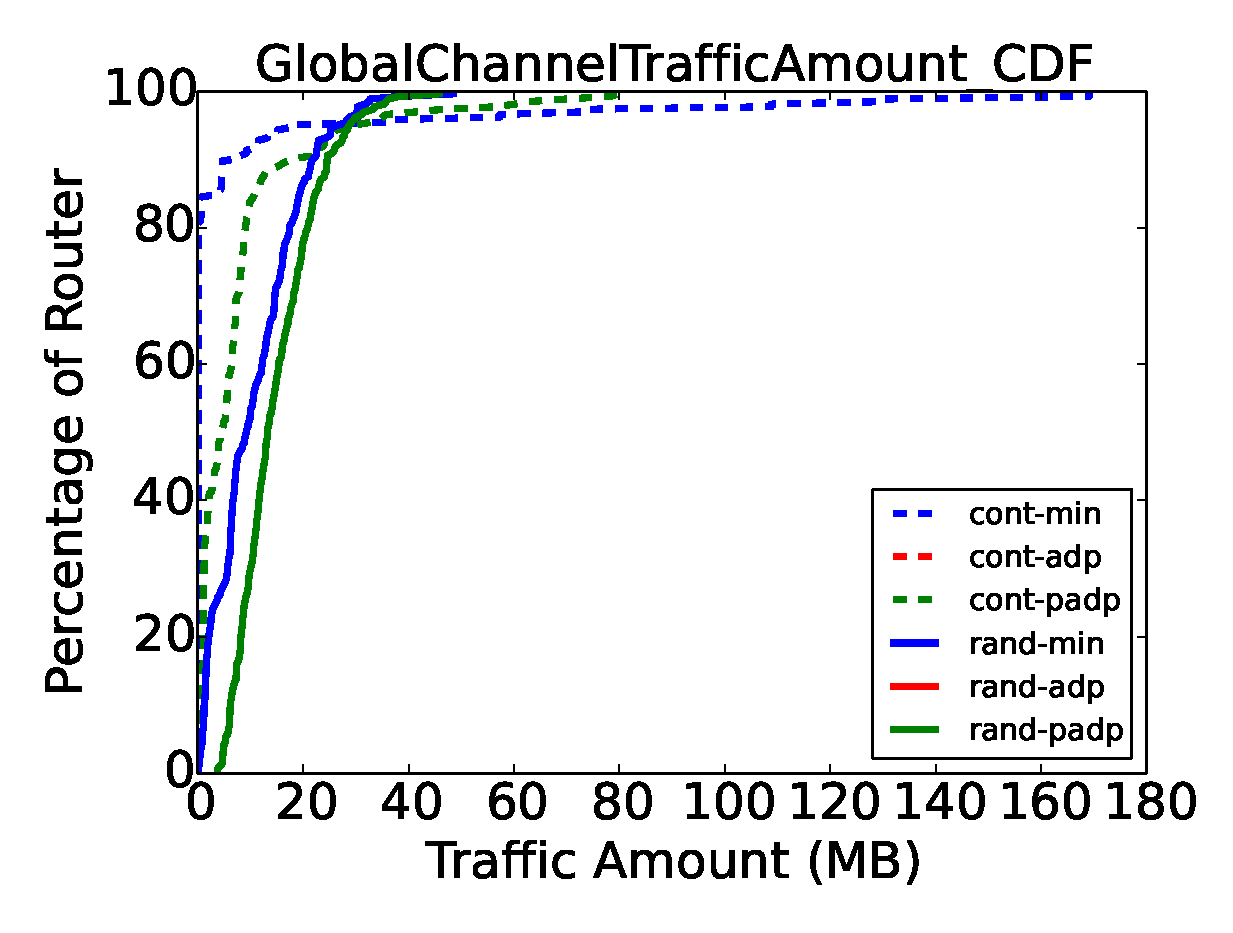
\includegraphics[height=1.8 in]{wkld/gc-traffic}
        \caption{Global Channel Traffic}
        \label{fig:global-channel-traffic}
    \end{subfigure}\hfill
    \hspace{1em}%
    \begin{subfigure}[t]{0.32\textwidth}
        \centering
        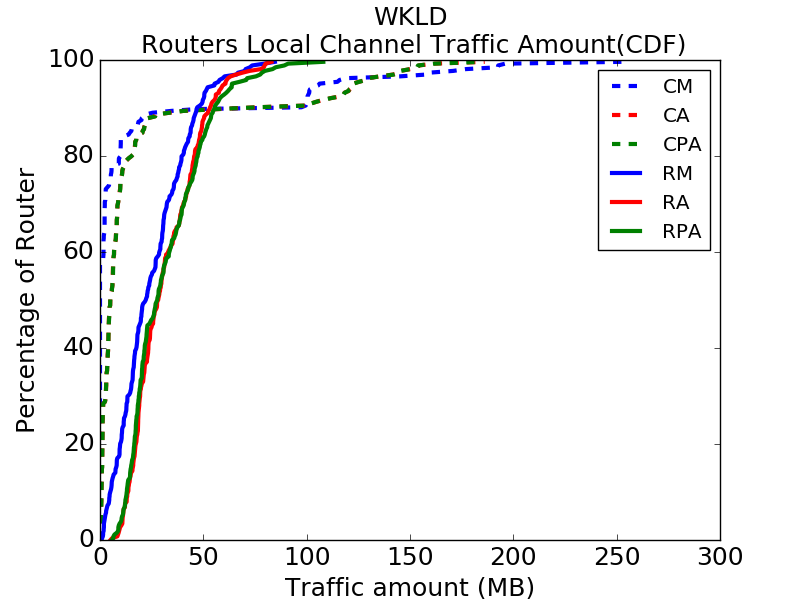
\includegraphics[height=1.8 in]{wkld/lc-traffic}
        \caption{Local Channel Traffic}
        \label{fig:local-channel-traffic}
    \end{subfigure}\hfill
    \hspace{1em}%
    \begin{subfigure}[t]{0.32\textwidth}
        \centering
        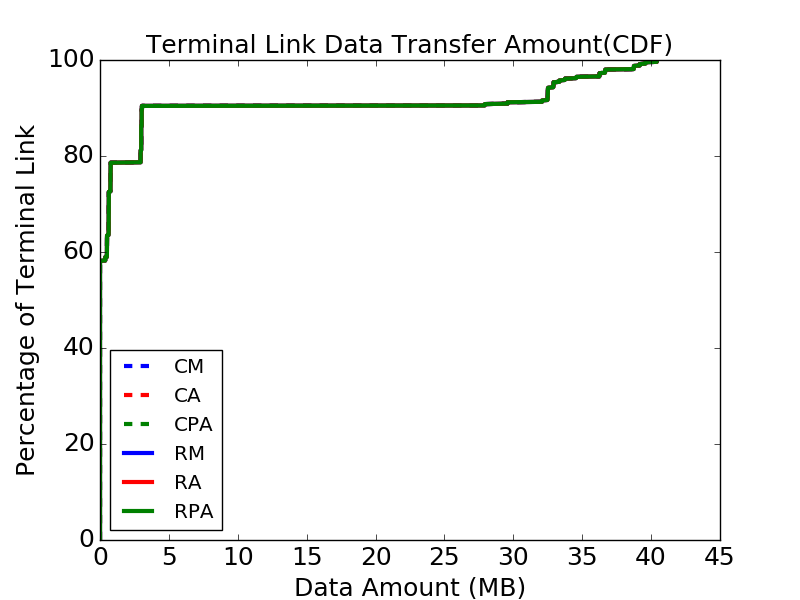
\includegraphics[height=1.8 in]{wkld/tl-traffic}
        \caption{Terminal Link Traffic}
        \label{fig:terminal-link-traffic}
    \end{subfigure}\\

    \centering   
    \begin{subfigure}[t]{0.32\textwidth}
        \centering
        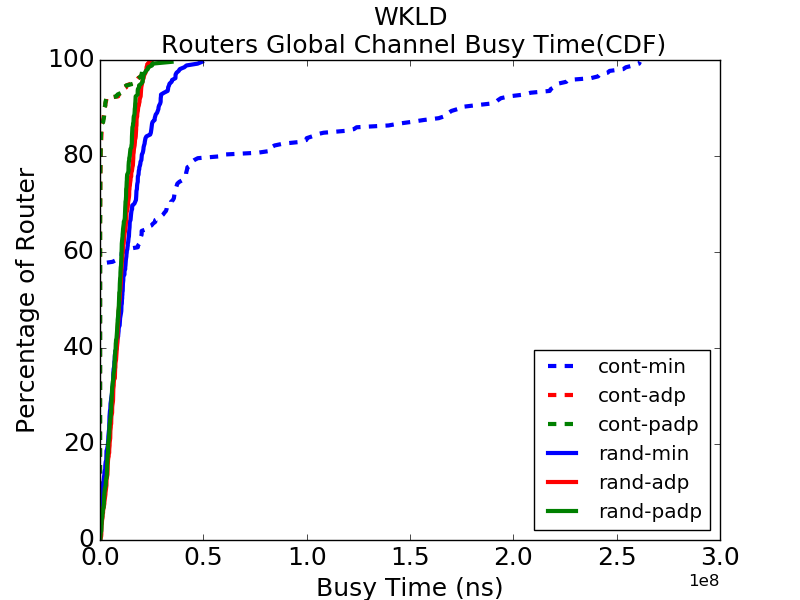
\includegraphics[height=1.8 in]{wkld/gc-stime}
        \caption{Global Channel Saturation Time}
        \label{fig:global-channel-stime}
    \end{subfigure}\hfill
     \hspace{1em}%
    \begin{subfigure}[t]{0.32\textwidth}
        \centering
        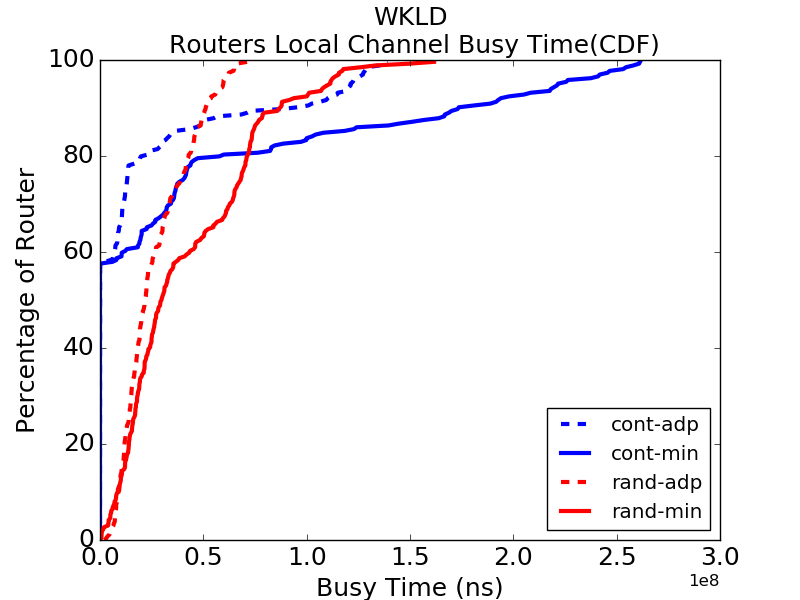
\includegraphics[height=1.8 in]{wkld/lc-stime}
        \caption{Local Channel Saturation Time}
        \label{fig:local-channel-stime}
    \end{subfigure}\hfill
    \hspace{1em}%
    \begin{subfigure}[t]{0.32\textwidth}
        \centering
        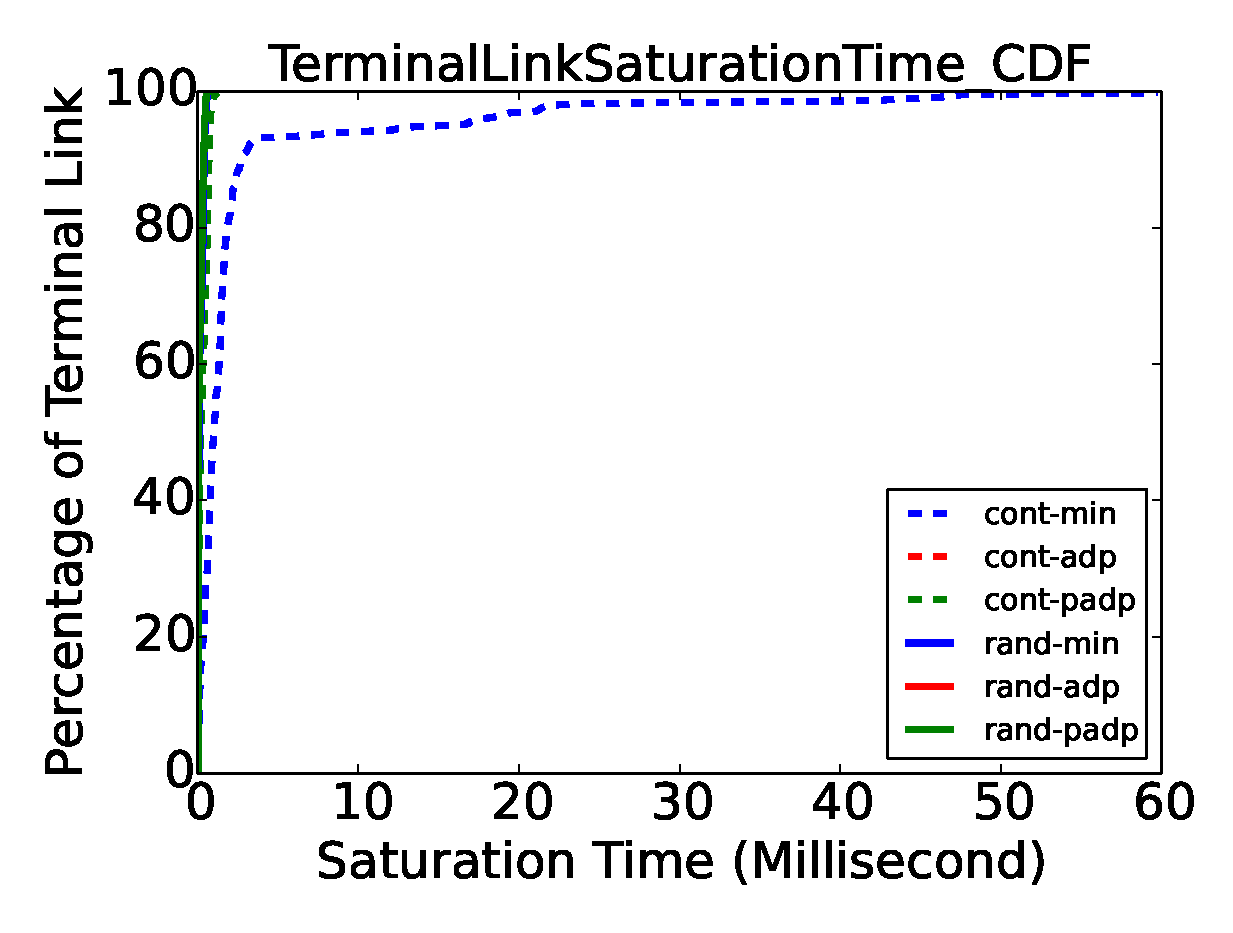
\includegraphics[height=1.8 in]{wkld/tl-stime}
        \caption{Terminal Link Saturation Time}
        \label{fig:terminal-link-stime}
    \end{subfigure}%
    \caption{Aggregate traffic and saturation time for Workload~\Rmnum{1} under the configurations listed in Table~\ref{tab: placement routing configs}. ``CA'' and ``CPA'' have equivalent behavior.}
   \label{fig:wkld-network-traffic-stime}
\end{figure*}


Figure~\ref{fig:wkld-network-traffic-stime} shows the aggregate traffic for terminal links, local and global channels,
as well as the corresponding saturation time for Workload~\Rmnum{1} under the placement and routing configurations summarized in Table~\ref{tab: placement routing configs}.
%explain CM
When contiguous placement is coupled with minimal routing (CM), 
application traffic is confined within the consecutively allocated groups, 
causing congestion on some routers along minimal paths to and from application nodes. 
Both local and global channels experience significant congestion, as applications span multiple groups.
Similarly, the saturation time for both local and global channels are also the highest compared with other configurations.
%explain CA and CPA
When contiguous placement is coupled with adaptive (CA) and progressive adaptive (CPA) routing, 
traffic is able to take non-minimal paths via intermediate routers, helping to alleviate congestion along the minimal paths. 
The resulting traffic through the most utilized local and global channels are greatly reduced, 
as shown in Figures~\ref{fig:global-channel-traffic} and~\ref{fig:local-channel-traffic}. \TODO{Traffic is not substantially reduced for local channel traffic}.
Similarly, the corresponding saturation time on local and global channels is also reduced significantly, 
demonstrating the efficacy of adaptive routing in this case. \TODO{How do we explain the similar distribution of traffic on local channels compared to the dissimilar distribution of saturation time?}
For contiguous placement, we see no perceptible difference in behavior between adaptive and progressive adaptive routing.


%Explain RM
In most cases for this study, the random placement policy behaves similarly across routing policies.
Random placement uniformly distributes MPI ranks over the network, 
balancing the resulting traffic load. 
As shown in Figures~\ref{fig:global-channel-traffic} and~\ref{fig:local-channel-traffic}, 
no router suffers exceptionally high volume of traffic on its local and global channels. 
When random placement is coupled with minimal routing (RM), less traffic is generated on account of
the packets avoiding intermediate forwarding. At the same time, there is still significant congestion on local channels due to the lack of ability of packets to traverse non-minimal routes, falling into the same trap as the contiguous-minimal configuration.
\TODO{check this}
%Explain RA, RPA
Coupled with (progressive) adaptive routing,
no router suffers exceptionally long saturation times on their global channels when random placement is in use, 
as shown in Figure~\ref{fig:global-channel-stime} and~\ref{fig:local-channel-stime}. Further, in comparison to contiguous allocations, random allocations result in a more evenly distributed load on the resulting channels, as expected.

% Explain terminal link traffic and busy time
Figures~\ref{fig:terminal-link-traffic} and \ref{fig:terminal-link-stime} are presented for the purpose of symmetry, 
showing the traffic per terminal link as well as the saturation time experienced at each terminal.
The terminal traffic distribution corresponds directly to application traffic, as we are using one MPI rank per node (terminal).
However, saturation times are different, resulting from the aforementioned network behavior. Particularly, contiguous allocations coupled with minimal routing results in a ``long-tail`` distribution of saturation time.

%===========================================================
%from the workload perspective to study the network performance. 
%The efficiency of the workload communication is another perspective to evaluate the network performance. 
%The average communication time spent by all MPI ranks when Workload~\Rmnum{1} is running under different placement and routing configurations shown in Table~\ref{tab:wkld-commtime}. 
%The random placement policy performs comparably with all routing policies (RM, RA and RPA). They outperform all contiguous placement configurations (CM, CA and CPA). The contiguous placement coupled with minimal routing (CM) results in highest communication time. When coupled with (progressive) adaptive routing (CA, CPA), the average communication time can be greatly reduced. When random placement is in use, the workload communication efficiency can be further improved. 
%
%
%\begin{table}[ht]
%\begin{center}
%\caption{Average communication time by all MPI ranks when Workload I is running on the dragonfly network under six different placement and routing configurations.} 
%\label{tab:wkld-commtime}
%\begin{tabular}{l c c c c c c }
%\toprule % Top horizontal line
%\toprule
%&\multicolumn{6}{c}{Placement and Routing Configurations} \\ 
%\cmidrule(l){2-7}
%          & CM & CA & CPA & RM & RA & RPA \\ % Column names row
%\midrule % In-table horizontal line
%Time(ms)  & 476  & 300  & 301  & 255  & 265  & 264  \\ % Content row 1
%
%\midrule % In-table horizontal line
%\bottomrule % Bottom horizontal line
%\end{tabular}
%\end{center}
%\end{table}
%
%
%The random placement can balance the network traffic load by uniformly distribute the traffic. The (progressive) adaptive routing can avoid the hot-spots by redirecting the traffic away from congested area. The network can reach its optimal performance, when random placement coupled with (progressive) adaptive routing are in use. 
%



\subsection{Individual Application Analysis}
\label{sec: workload-1 app analysis}

\begin{figure*}[t!]
    \centering
    \begin{subfigure}[t]{0.32\textwidth}
        \centering
        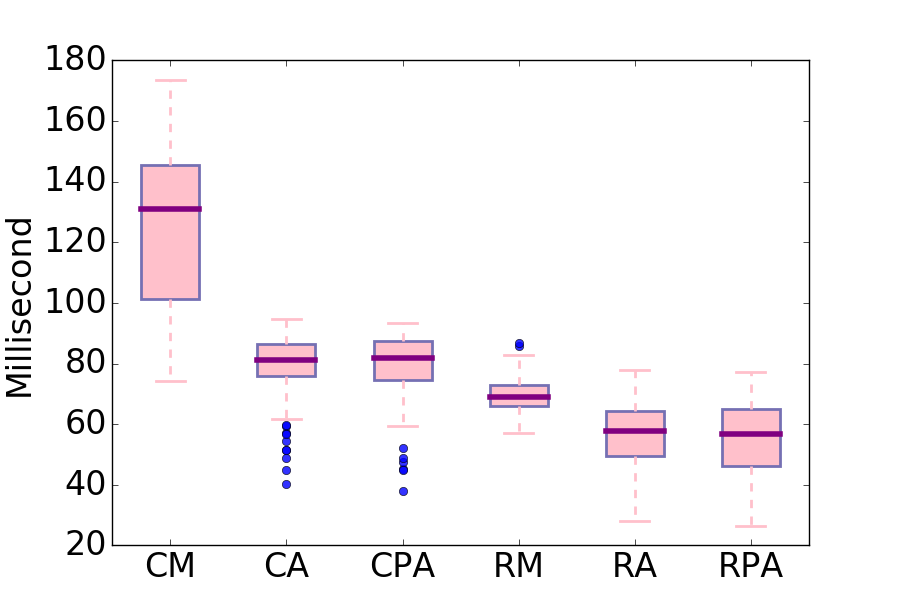
\includegraphics[height=1.5 in]{wkld/mg/commtime}
        \caption{MultiGrid}
        \label{fig:mg-commtime}
    \end{subfigure}%
    \hspace{1em}%
    \begin{subfigure}[t]{0.32\textwidth}
        \centering
        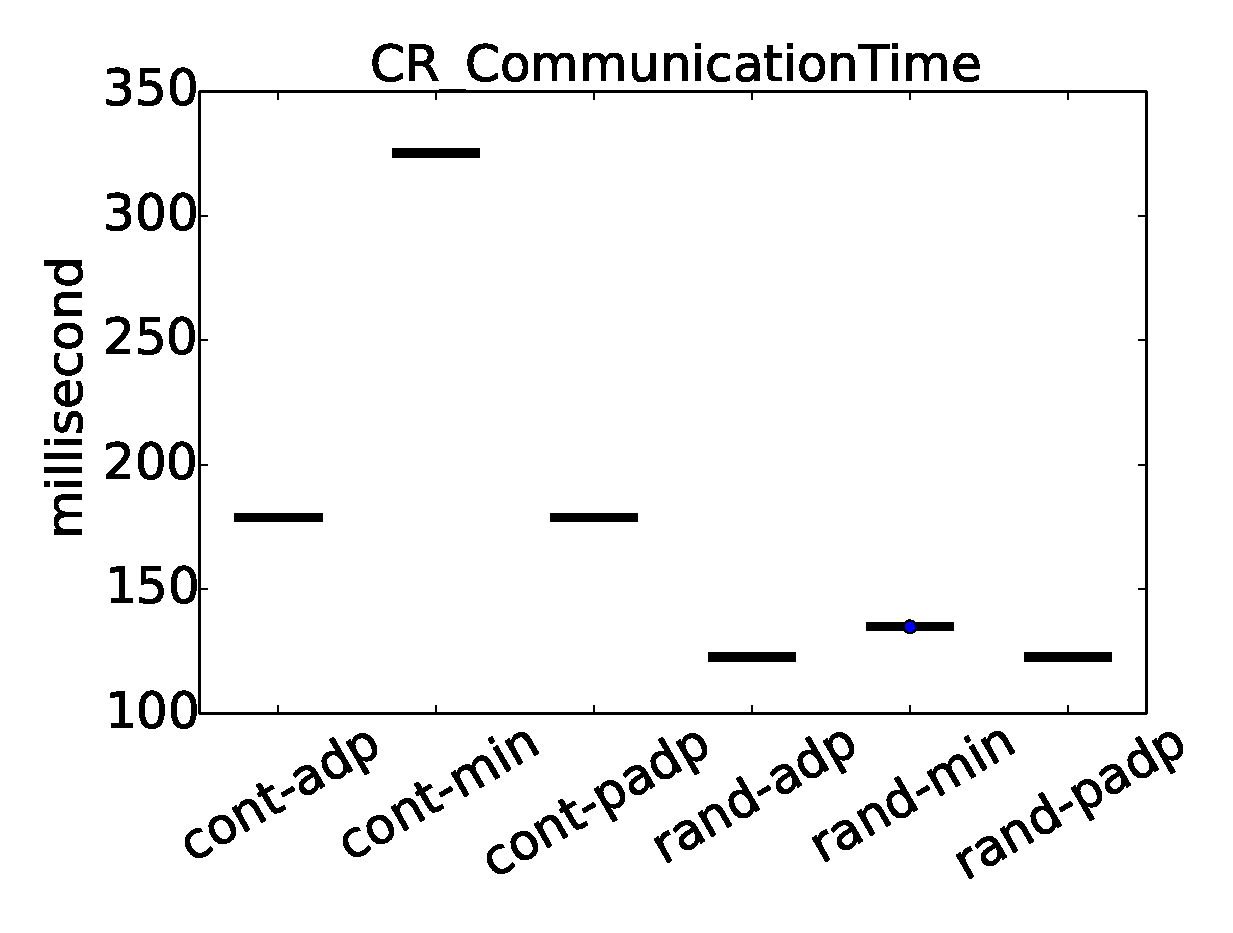
\includegraphics[height=1.5 in]{wkld/cr/commtime}
        \caption{CrystalRouter}
        \label{fig:cr-commtime}
    \end{subfigure}%
    \hspace{1em}%
    \begin{subfigure}[t]{0.32\textwidth}
        \centering
        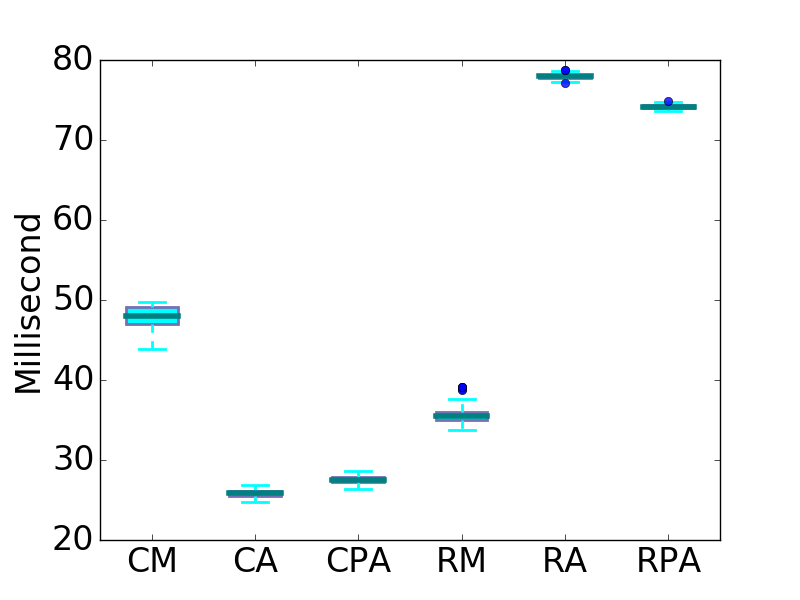
\includegraphics[height=1.5 in]{wkld/amg/commtime}
        \caption{AMG}
        \label{fig:amg-commtime}
    \end{subfigure}%
    \caption{Communication time distribution across application ranks in Workload~\Rmnum{1}.}
   \label{fig:apps-commtime}
\end{figure*}

Now that the system-level view has been analyzed, we turn to evaluate the
behavior of each application within Workload~\Rmnum{1}.
Figure~\ref{fig:apps-commtime} shows the communication time distribution across
application ranks for different placement and routing configurations.

The relative behavior of contiguous allocations is roughly similar in all three
applications. Contiguous placement with minimal routing results in poor relative
performance across the board compared to the adaptive routing alternatives.
Given the analyses in Section~\ref{sec: workload-1 network analysis}, this is to
be expected -- the contiguous-minimal configuration results in significant
congestion.

For the MultiGrid and CrystalRouter applications (Figures~\ref{fig:mg-commtime} and
\ref{fig:cr-commtime}, respectively), using random allocation with any routing
method results in performance improvements over contiguous allocations, which is
largely in agreement with previous work (see Section~\ref{sec:related work}).
\TODO{did previous work make this strong a claim?}. The high-radix nature of the
network topology ensures that the benefits from the resulting load balancing
outweigh the costs of extra hops for point-to-point messages.

The AMG application (Figure~\ref{fig:amg-commtime}), however, shows markedly
different behavior when using random allocation. Random allocation with minimal
routing results in worse performance than contiguous-adaptive configurations,
while using adaptive routing results in significant performance regressions. As
this is a counterintuitive result not reached by other works, we investigate
further.

\begin{comment} JJ - doing some reorg, so keeping the old text just in case
Now that the system-level view has been analyzed, we turn to evaluate the behavior of each application within Workload~\Rmnum{1}.
Figure~\ref{fig:apps-commtime} shows the communication time distribution across application ranks for different placement and routing configurations.
As shown in Figure~\ref{fig:mg-commtime}, 
MultiGrid takes the most communication time when it is running with contiguous placement and minimal routing (CM). 
When contiguous placement coupled with adaptive or progressive adaptive routing (CA, CPA) are in use, 
the communication time is significantly reduced. 
Random placement coupled with minimal routing (RM) can make further improvement, 
and reaches the best performance(lowest communication time) when coupled with adaptive and progressive adaptive routing(RA, RPA). 
Due to the variance of data transfer amount among MPI ranks, 
MultiGrid communication time also presents great variation, 
indicating by the long boxes in Figure~\ref{fig:mg-commtime}.

CrystalRouter takes more communication time compared with the other applications because of its high volume of data transfer. 
When it is running with six placement and routing configurations, 
CrystalRouter communication time presents similarly trend as MultiGrid but with little variance, shown in Figure~\ref{fig:cr-commtime}. 


AMG is quite an exception. 
The communication time of AMG running with different placement and routing configuration are shown in Figure~\ref{fig:amg-commtime}.
When contiguous placement is in use, AMG behaves similarly as MultiGrid and CrystalRouter over three routing policies. 
It takes comparable amount of communication time when contiguous placement coupled with adaptive and progressive routing. 
When coupled with minimal routing, the communication time almost doubles. 
The communication time skyrockets when random placement coupled with (progressive) adaptive routing (RPA, RA) are in use. Minimal routing (RM) can mitigate this performance degradation, but still worse than CA and CPA. We observe that when Workload~\Rmnum{1} is running with random placement and (progressive) adaptive routing, 
the performance of MultiGrid and CrystalRouter are significant improved, whereas AMG suffers performance degradation. 
\end{comment}


\begin{figure*}[t]
    \centering
    \begin{subfigure}[t]{0.32\textwidth}
        \centering
        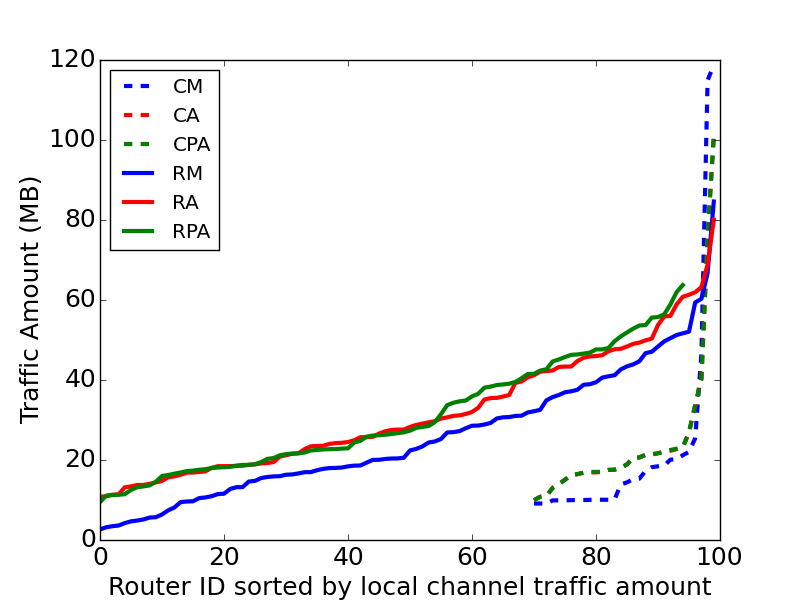
\includegraphics[height=1.8 in]{wkld/mg/lc-traffic}
        \caption{MultiGrid Local Channel Traffic}
        \label{fig:mg-lc-traffic}
    \end{subfigure}\hfill
    \begin{subfigure}[t]{0.32\textwidth}
        \centering
        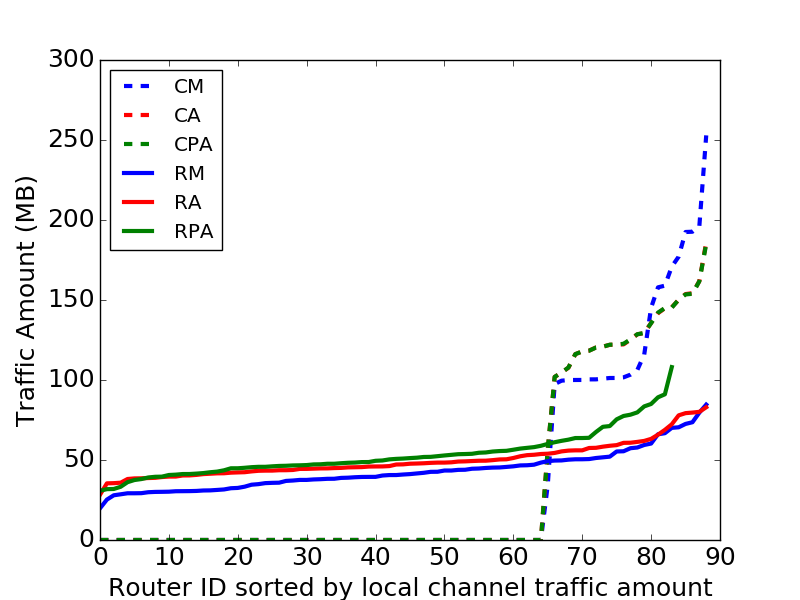
\includegraphics[height=1.8 in]{wkld/cr/lc-traffic}
        \caption{CrystalRouter Local Channel Traffic}
        \label{fig:cr-lc-traffic}
    \end{subfigure}\hfill
    \begin{subfigure}[t]{0.32\textwidth}
        \centering
        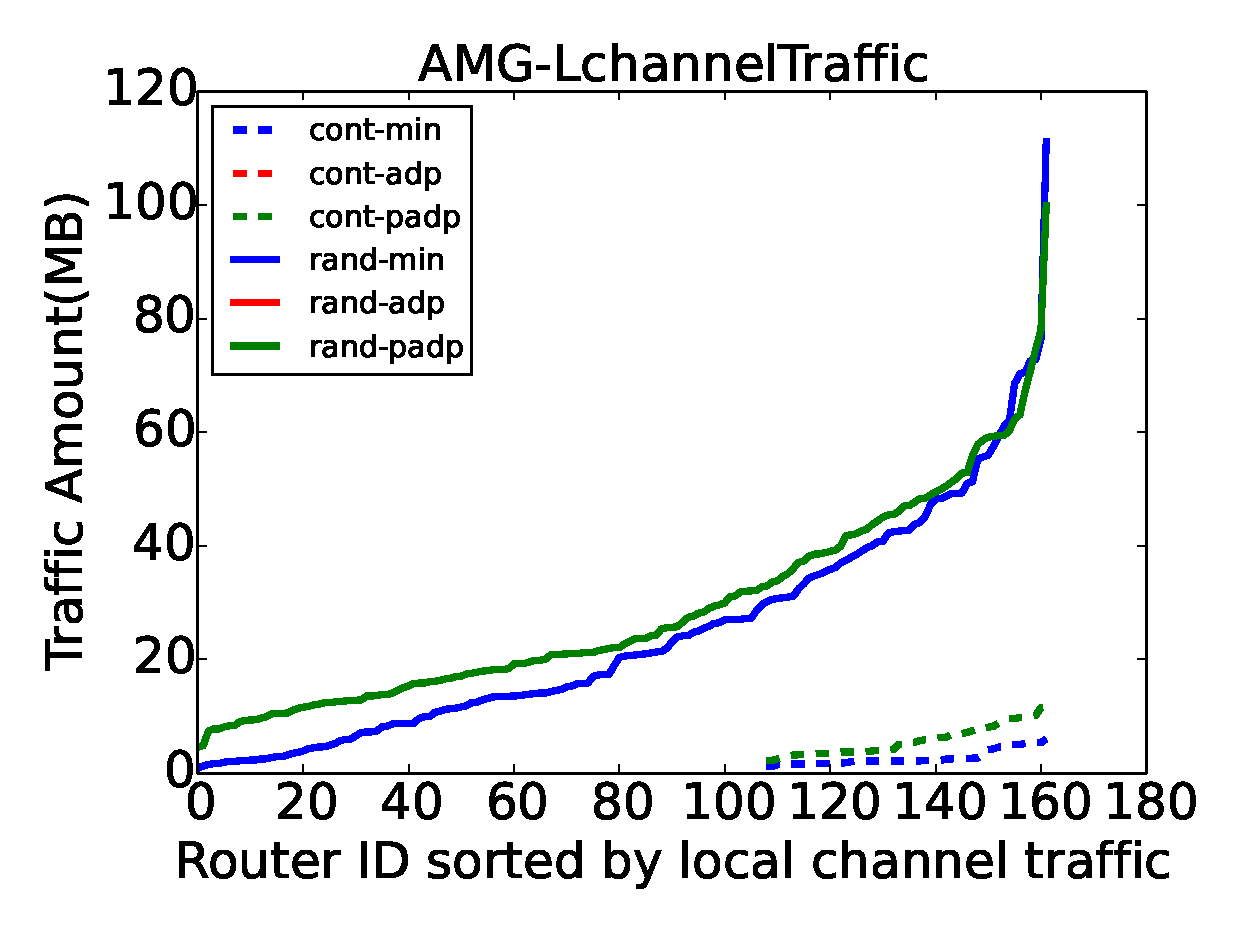
\includegraphics[height=1.8 in]{wkld/amg/lc-traffic}
        \caption{AMG Local Channel Traffic}
        \label{fig:amg-lc-traffic}
    \end{subfigure}\\  
    \centering
   \begin{subfigure}[t]{0.32\textwidth}
        \centering
        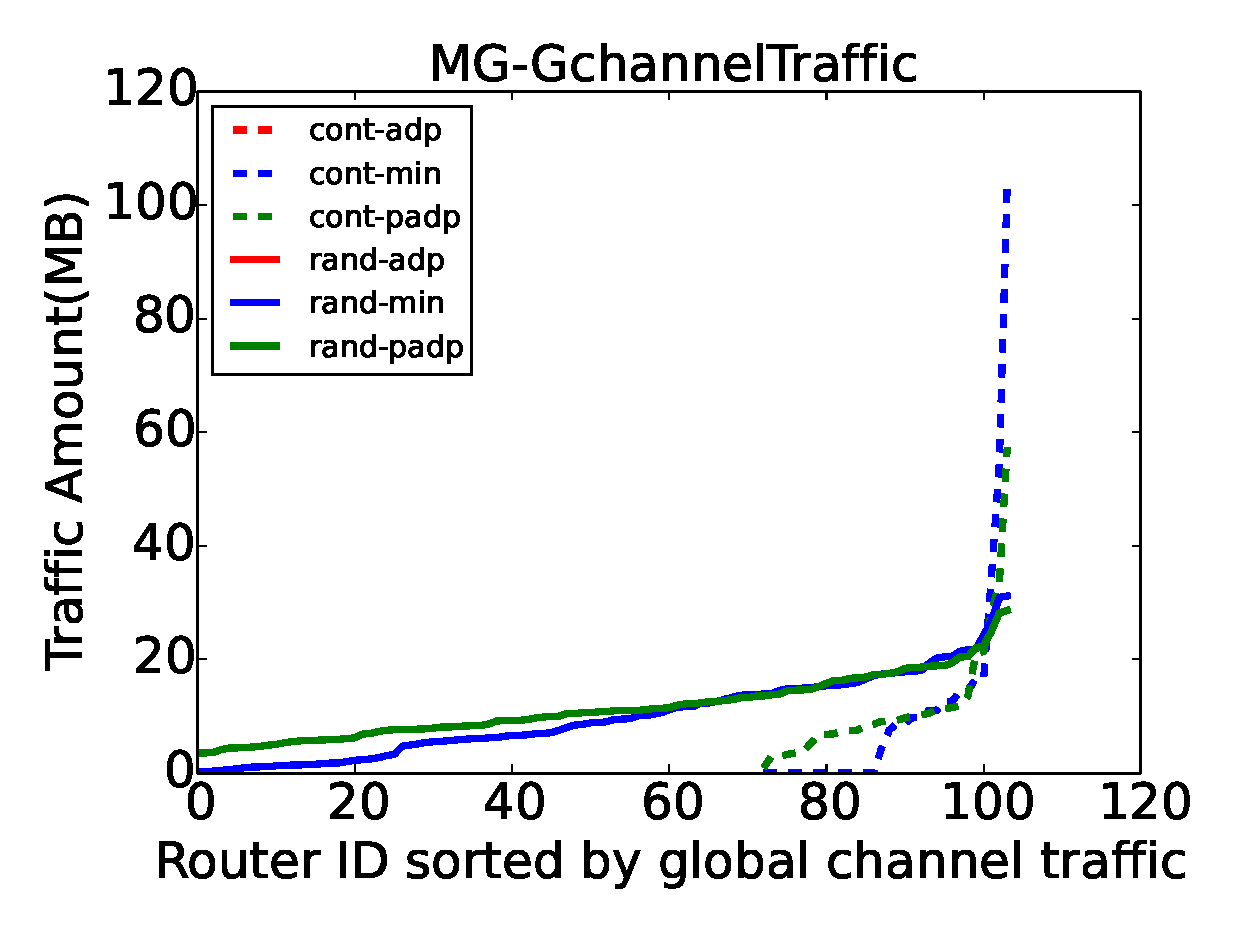
\includegraphics[height=1.8 in]{wkld/mg/gc-traffic}
        \caption{MultiGrid Global Channel Traffic}
        \label{fig:mg-gc-traffic}
    \end{subfigure}\hfill
    \begin{subfigure}[t]{0.32\textwidth}
        \centering
        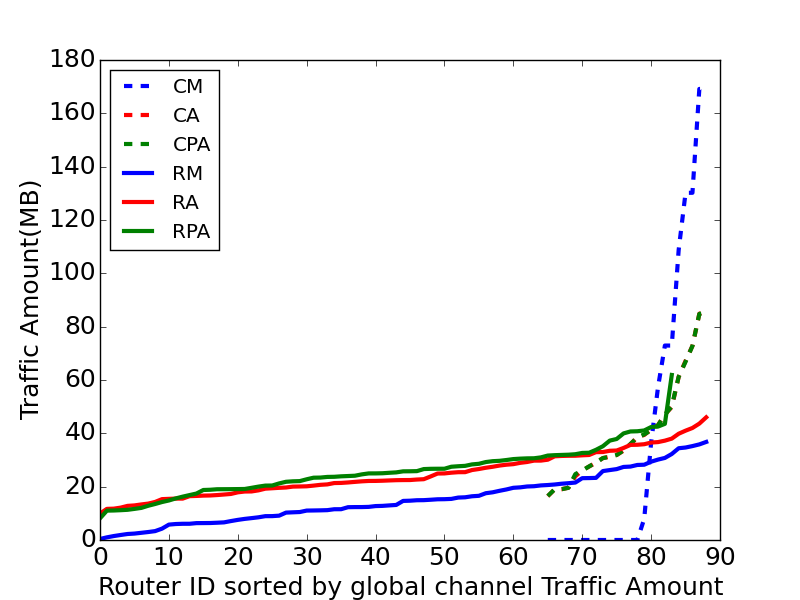
\includegraphics[height=1.8 in]{wkld/cr/gc-traffic}
        \caption{CrystalRouter Global Channel Traffic}
        \label{fig:cr-gc-traffic}
    \end{subfigure}\hfill
    \begin{subfigure}[t]{0.32\textwidth}
        \centering
        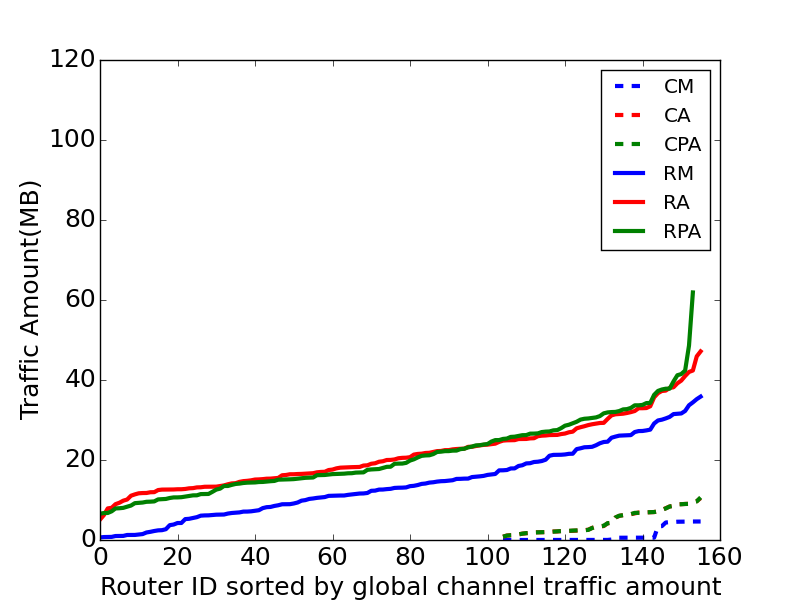
\includegraphics[height=1.8 in]{wkld/amg/gc-traffic}
        \caption{AMG Global Channel Traffic}
        \label{fig:amg-gc-traffic}
    \end{subfigure}
   \caption{Aggregate workload traffic for routers serving specific applications. ``CA'' and ``CPA'' have equivalent behavior. More routers are involved in serving each application when random placement is in use, compared to contiguous placement.}
   \label{fig:3app-lc-gc-traffic}
\end{figure*}

% Show the evidence from network level, explain why AMG is different. 

We step back to a network-level system view to identify the culprit behind AMG's
abnormal behavior with random placement. This time, however, we identify the
compute nodes that each MPI rank resides on and the routers that are serving
each application, and analyze the traffic on a per-application basis.  The
results of this experimentation are presented in
Figure~\ref{fig:3app-lc-gc-traffic}. Note that different numbers of routers are
used in the contiguous and random allocation configurations, as each router
serves multiple terminals.

The system behavior with respect to the CrystalRouter application arguably best
matches expectations. Use of contiguous allocations result in a subset of
channels with a significant traffic load while a significant portion are
unused. Use of random allocations result in a comparatively smoother traffic
distribution, with some variation on the margins due to the randomness.

MultiGrid shows roughly similar behavior for contiguous allocations, but
different behavior along the local channels. There is a significant variation in
the traffic distribution of local channels, even with adaptive routing, which
should have the net effect of distributing said traffic.

AMG shows a similar level of variation to MultiGrid in this case. However, it is
the least communication-intensive application of the three by a significant
factor. In effect, the routers serving the AMG application are being utilized by
MultiGrid and CrystalRouter, resulting in AMG traffic queuing up in their
respective routers. Since the relative traffic is so low, AMG ends up
experiencing significant slowdowns due to this effect. We refer to this phenomenon
as AMG being ``bullied" by MultiGrid and CrystalRouter.

\begin{comment} JJ - some more reorg here, also a few of the observations don't match the data

The routers serving MultiGrid and CrystalRouter have a high traffic volume on both local and global channels when contiguous placement is in use, 
shown as the dashed line in Figure~\ref{fig:mg-lc-traffic},~\ref{fig:mg-gc-traffic} and Figure~\ref{fig:cr-lc-traffic},~\ref{fig:cr-gc-traffic}. 
On the other hand, the random placement can uniformly distribute the traffic of MultiGrid and CrystalRouter over the network, 
alleviate local congestion and balance the traffic load among all routers, 
shown as the solid lines in Figure~\ref{fig:mg-lc-traffic},~\ref{fig:mg-gc-traffic} and Figure~\ref{fig:cr-lc-traffic},~\ref{fig:cr-gc-traffic}. 
MultiGrid and CrystalRouter benefit from random placement by getting their high volume of traffic being redirected 
from their over-loaded routers to the less busy routers in the network. 
In this case, a majority of those less busy routers are belonging to AMG.


Since AMG is less communication-intensive, 
the routers serving AMG have small volume of traffic on local and global channels when the contiguous placement is use, 
shown as the dashed line in Figure~\ref{fig:amg-lc-traffic},~\ref{fig:amg-gc-traffic}. 
When random placement is in use, 
more routers are involved in serving AMG, 
and the traffic skyrockets on the local and global channels, 
shown as the solid lines in Figure~\ref{fig:amg-lc-traffic},~\ref{fig:amg-gc-traffic}. 
The increased traffic comes from the communication-intensive MultiGrid and CrystalRouter. 
AMG behaves abnormally when random placement is in use 
because the routers serving AMG have to take the traffic from MultiGrid and CrystalRouter. 
The extra traffic from the other communication-intensive applications 
takes advantage the network resources belonging to AMG and slows down AMG's communication. 
We refers this phenomenon as AMG being ``bullied" by MultiGrid and CrystalRouter.
\end{comment}


\subsection{Key Observations}
\label{sec:workload-1-observations}

In summary, based on the simulations presented in Section~\ref{sec: workload-1 network analysis} and \ref{sec: workload-1 app analysis}, we have made the following observations.

\emph{System-level performance is significantly improved when random placement and adaptive routing are in use.} 
Random placement can uniformly distribute MPI ranks of application over the network, 
and adaptive routing can redirect the traffic from congested routers to other less busy routers. 
The combination of the two minimizes hot-spots and promotes load-balanced distribution. The resulting increased number of hops per message was not a significant detriment in comparison. This matches what is seen in the literature.

\emph{The performance of communication-intensive jobs in the system improves using a random allocation policies}
Both CrystalRouter and MultiGrid, the two most communication-intensive jobs,
both saw improved distributions of communication performance when moving to a
random allocation. Again, this matches what is seen in the literature.

\emph{The performance of less communication-intensive jobs in workload regresses when random placement and adaptive routing are in use.} 
AMG in Workload~\Rmnum{1} are ``bullied" by its concurrently running communication-intensive peers, MultiGrid and CrystalRouter.
AMG shares routers and groups with MultiGrid and CrystalRouter under random placement. 
The traffic from MultiGrid and CrystalRouter is (re)directed to the routers that serve AMG, 
slowing down AMG's communication. 
\footnote{We have tried three different congestion ``sensing'' schemes in the literature for adaptive routing~\cite{won-prog-adaptive}. Although there are some variations between the results, none of the congestion sensing scheme prevent the ``bully'' behavior.}

\emph{In contrast, performance consistency of each application is achieved only when contiguous placement and minimal routing are in use.} 
As a corollary to the previous observation, router and group sharing among applications are guaranteed to be prohibited when using contiguous placement with minimal routing (sharing of spare nodes within a group notwithstanding). This renders the ``bully'' behavior moot, though with the downside of significant performance degradation, so such approaches must be carefully considered.
\TODO{not sure whether to keep this -- we don't really talk about performance consistency in the preceding text. It's a valid observation, though, so it should be somewhere...} 




\section{Study of Parallel Workload \Rmnum{2 }}
%\section{``Bully" become ``bullied"}
\label{sec:workload-2}

In this section, we use a different experimental configuration to verify and
explore the observations made in the previous section. Specifically, we conduct
the same sets of experiments through Workload~\Rmnum{2}, which consists of sAMG,
MultiGrid and CrystalRouter. By replacing AMG with sAMG, we turn the ``bully"
into the ``bullied".

\subsection{Network Performance Analysis}
\label{sec: workload-2 network analysis}

Figure~\ref{fig:synwkld-network-traffic-stime} shows aggregate traffic and
saturation times for Workload~\Rmnum{2}, corresponding to
Figure~\ref{fig:wkld-network-traffic-stime} in Workload~\Rmnum{1}.  Replacing
AMG with sAMg results in greater aggregate traffic as well as more saturation
than in Workload~\Rmnum{1}, but regardless, similar patterns can be observed.
Contiguous placement with minimal routing results in load imbalances with
respect to both traffic and saturation. The addition of adaptive routing
alleviates these effects to some degree, particularly with respect to global
channel usage, while trading off saturation in global channels for saturation in
the local channels. Using random placement again shows roughly similar performance
characteristics across routing configurations, with adaptive routing helping to
balance aggregate load while increasing the aggregate traffic due to the related
indirection.

\begin{figure*}[t]
    \centering
    \begin{subfigure}[t]{0.32\textwidth}
        \centering
        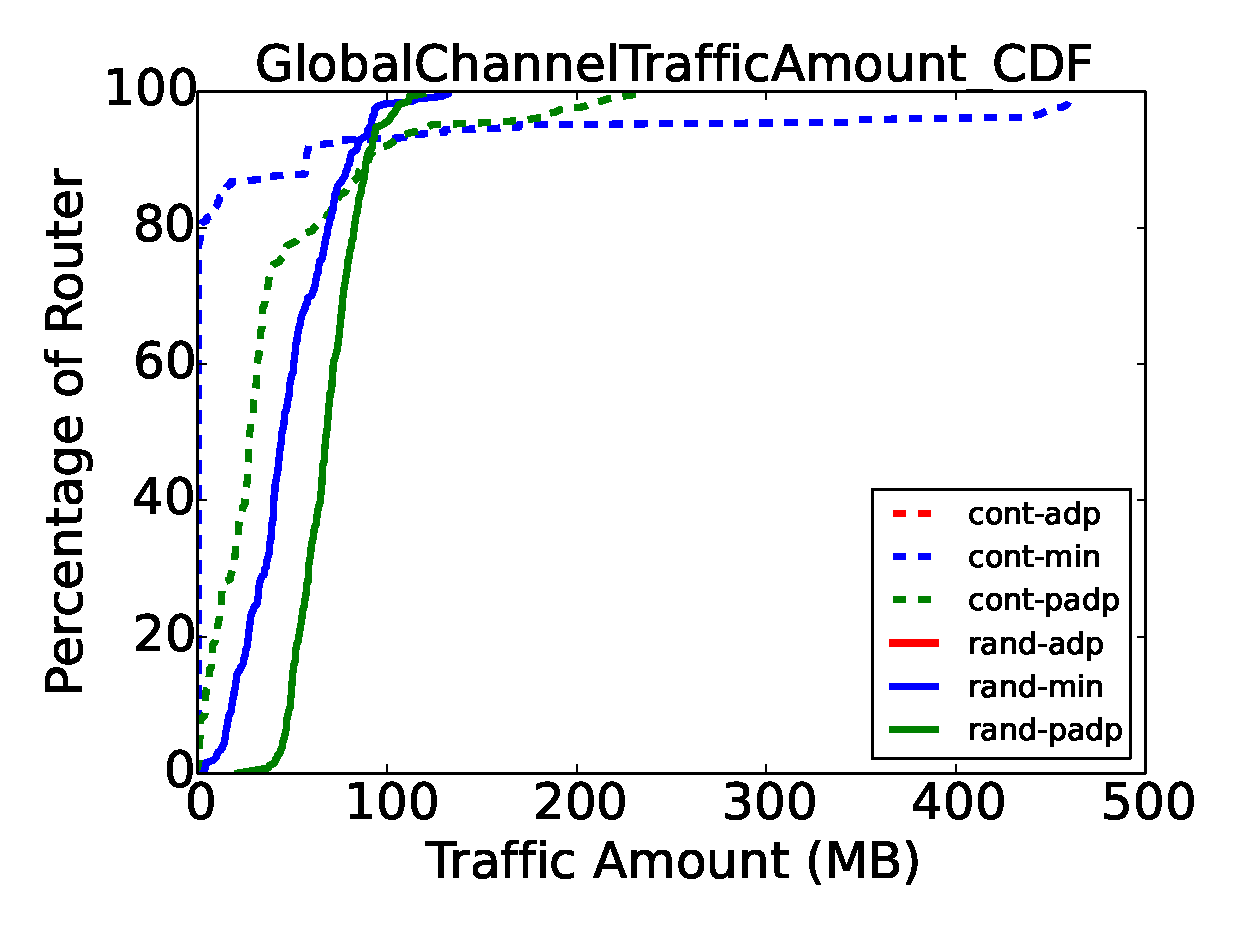
\includegraphics[height=1.8 in]{syn-wkld/gc-traffic}
        \caption{Global Channel Traffic}
        \label{fig:synwkld-global-channel-traffic}
    \end{subfigure}\hfill
    \hspace{1em}%
    \begin{subfigure}[t]{0.32\textwidth}
        \centering
        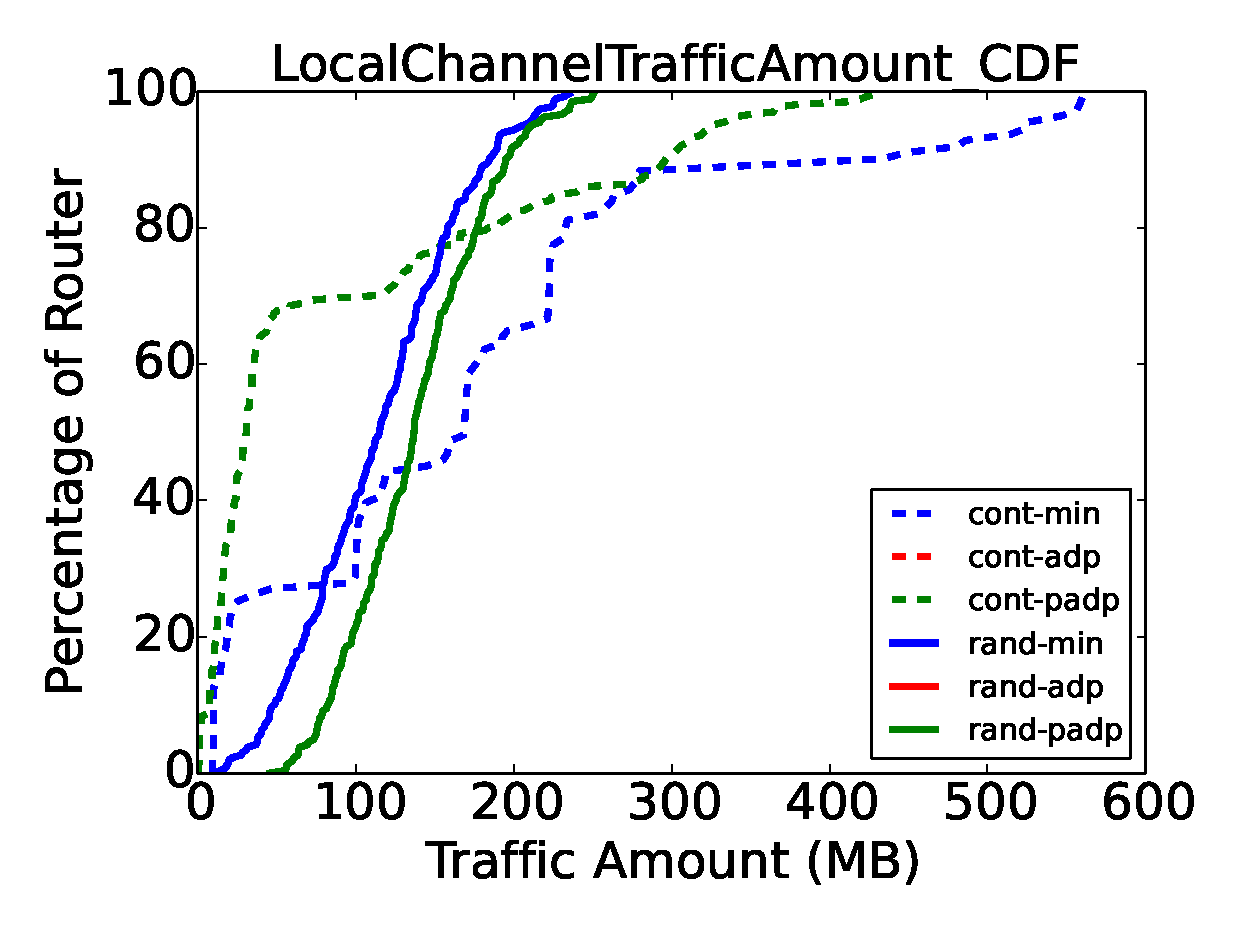
\includegraphics[height=1.8 in]{syn-wkld/lc-traffic}
        \caption{Local Channel Traffic}
        \label{fig:synwkld-local-channel-traffic}
    \end{subfigure}\hfill
    \hspace{1em}%
    \begin{subfigure}[t]{0.32\textwidth}
        \centering
        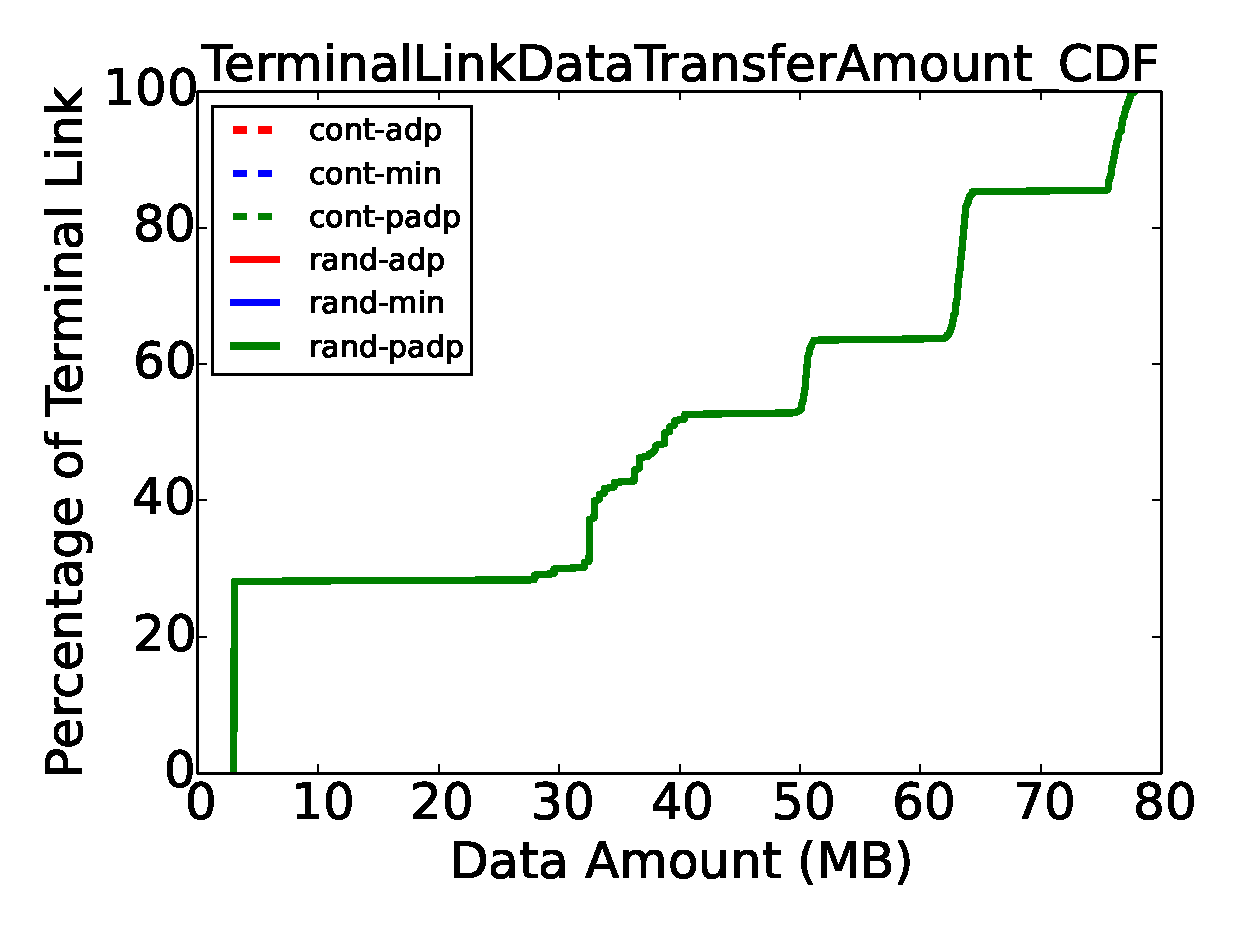
\includegraphics[height=1.8 in]{syn-wkld/tl-traffic}
        \caption{Terminal Link Traffic}
        \label{fig:synwkld-terminal-link-traffic}
    \end{subfigure}\\

    \begin{subfigure}[t]{0.32\textwidth}
        \centering
        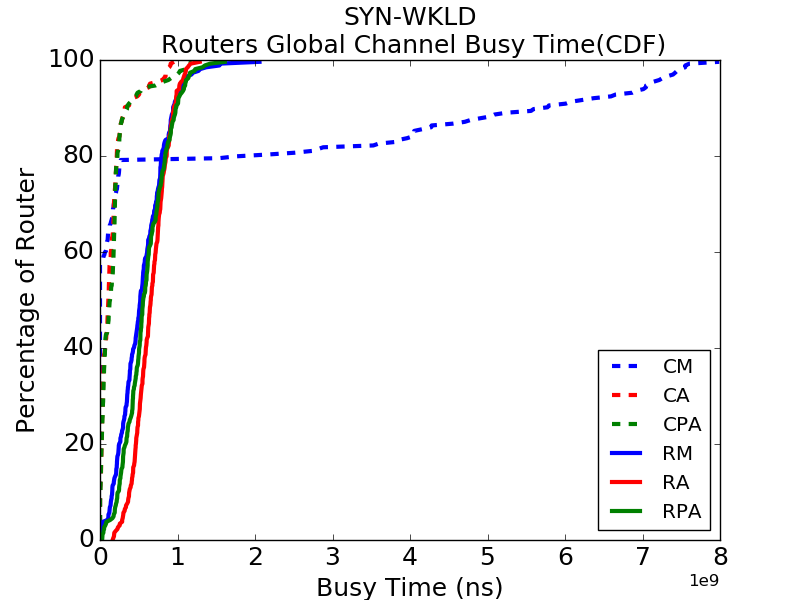
\includegraphics[height=1.8 in]{syn-wkld/gc-btime}
        \caption{Global Channel Saturation Time}
        \label{fig:synwkld-global-channel-stime}
    \end{subfigure}\hfill
     \hspace{1em}%
    \begin{subfigure}[t]{0.32\textwidth}
        \centering
        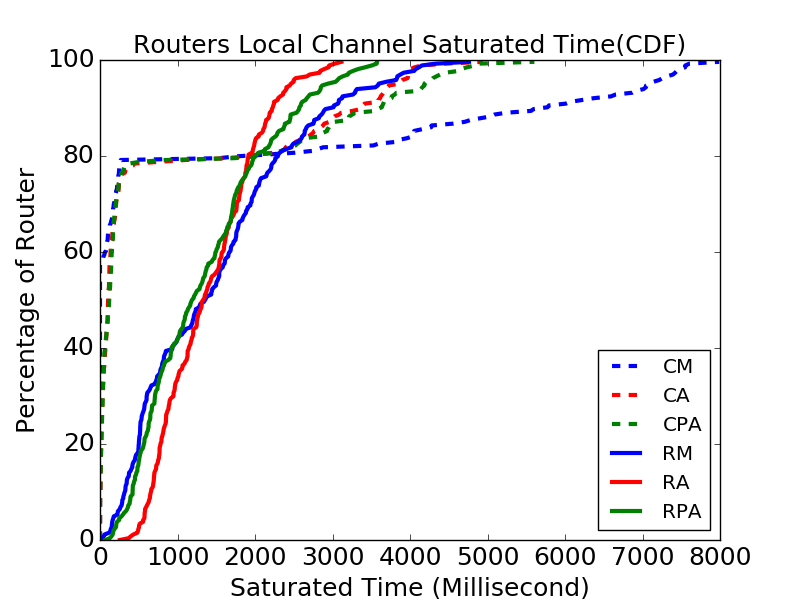
\includegraphics[height=1.8 in]{syn-wkld/lc-btime}
        \caption{Local Channel Saturation Time}
        \label{fig:synwkld-local-channel-stime}
    \end{subfigure}\hfill
    \hspace{1em}%
    \begin{subfigure}[t]{0.32\textwidth}
        \centering
        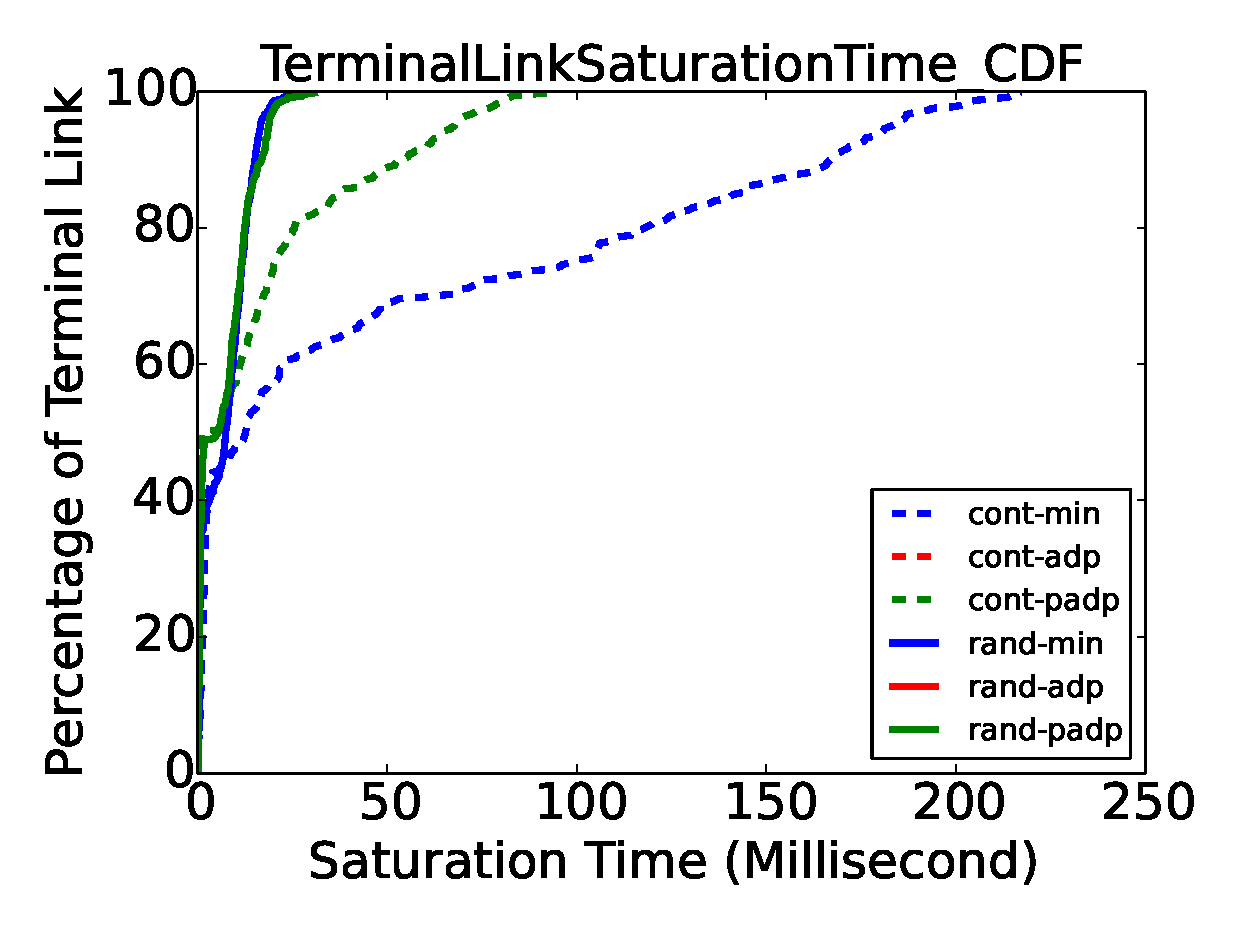
\includegraphics[height=1.8 in]{syn-wkld/tl-btime}
        \caption{Terminal Link Saturation Time}
        \label{fig:synwkld-terminal-link-stime}
    \end{subfigure}%
   \caption{Aggregate traffic and saturation time for Workload~\Rmnum{2} under the configurations listed in Table~\ref{tab: placement routing configs}.}
   \label{fig:synwkld-network-traffic-stime}
\end{figure*}


%+================================================================
%The average communication time spent by all MPI ranks when Workload~\Rmnum{2} is running under different placement and routing configurations shown in Table~\ref{tab:syn-wkld-commtime}. 
%We can observe the similar pattern as in Table~\ref{tab:wkld-commtime}
%The contiguous placement coupled with minimal routing results in highest communication time. 
%The random placement coupled with minimal routing is the most efficient. 
%Progressive adaptive routing is better than adaptive routing when random placement is in use, 
%and they have comparable results when coupled contiguous placement. 
%Same as Workload~\Rmnum{1}, the network reaches the optimal performance when Workload~\Rmnum{2} is running with random placement and adaptive routing. 
%
%\begin{table}[ht]
%\begin{center}
%\caption{Average time spent on communication by all MPI ranks when Workload II is running on dragonfly network under six different placement and routing configurations.} 
%\label{tab:syn-wkld-commtime}
%%\centering % Centers the table on the page, comment out to left-justify
%\begin{tabular}{l c c c c c c }
%\toprule % Top horizontal line
%\toprule
%&\multicolumn{6}{c}{Placement and Routing Configuration} \\ % Amalgamating several columns into one cell is done using the \multicolumn command as seen on this line
%\cmidrule(l){2-7}
%          & CM & CA & CPA & RM & RA & RPA \\ % Column names row
%\midrule % In-table horizontal line
%Time(ms)  & 3360 & 2204 & 2335 & 1791 & 2367 & 1965 \\ % Content row 1
%
%\midrule % In-table horizontal line
%\bottomrule % Bottom horizontal line
%\end{tabular}
%\end{center}
%\end{table}



\subsection{Individual Application Analysis}
\label{sec: workload-2 app analysis}

We study the performance of each application individually in the same manner as
in Section~\ref{sec: workload-1 app analysis}.
Figure~\ref{fig:syn-apps-commtime} shows the communication time distributions of
the ranks of the three applications, running concurrently in Workload~\Rmnum{2}.
The ``bully" in Workload~\Rmnum{1} becomes the ``bullied" in Workload~\Rmnum{2}. 
MultiGrid and CrystalRouter are in this instance the less communication-intensive applications. 
With random placement and (progressive) adaptive routing, 
MultiGrid and CrystalRouter experience prolonged communication time, 
as shown in Figure~\ref{fig:syn-mg-commtime}, \ref{fig:syn-cr-commtime}. 
On the other hand, sAMG (Figure~\ref{fig:syn-samg-commtime}) benefits from those configurations
in a similar manner to CrystalRouter in Workload~\Rmnum{1}.
Contiguous placement coupled with minimal routing, while preventing the bully
behavior, results in poor performance for all of the applications except CrystalRouter,
which we also expect is due to a higher degree of network isolation.

\begin{figure*}[t!]
    \centering
    \begin{subfigure}[t]{0.32\textwidth}
        \centering
        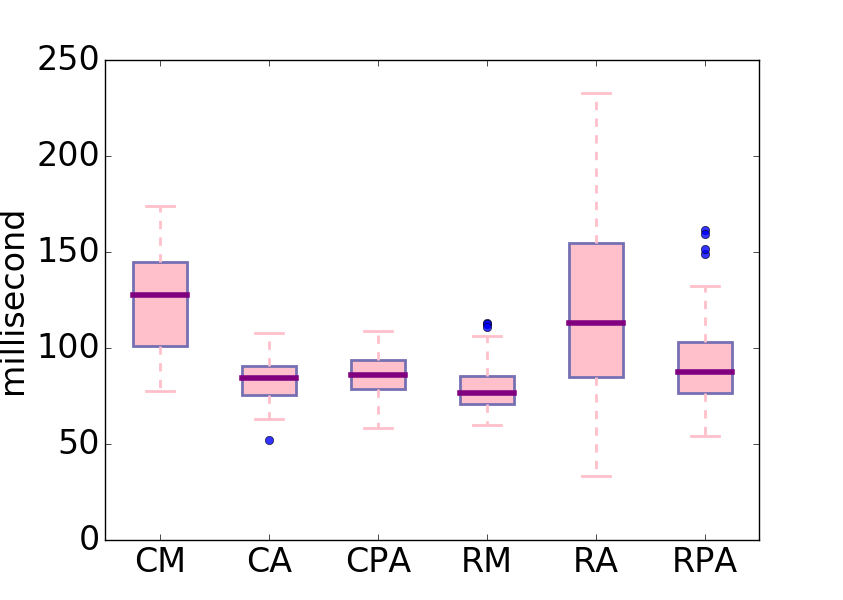
\includegraphics[height=1.5 in]{syn-wkld/mg/commtime}
        \caption{MultiGrid}
        \label{fig:syn-mg-commtime}
    \end{subfigure}%
    \begin{subfigure}[t]{0.32\textwidth}
        \centering
        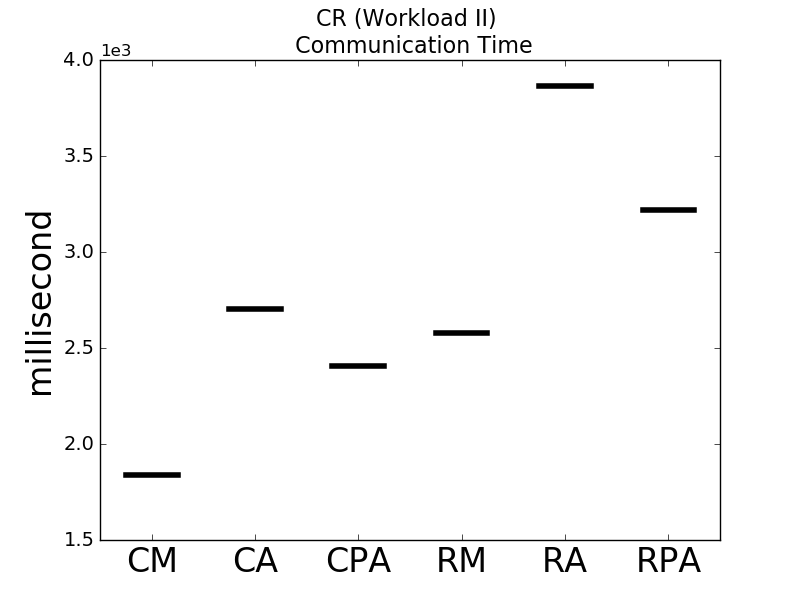
\includegraphics[height=1.5 in]{syn-wkld/cr/commtime}
        \caption{CrystalRouter}
        \label{fig:syn-cr-commtime}
    \end{subfigure}%
    \hspace{1em}%
    \begin{subfigure}[t]{0.32\textwidth}
        \centering
        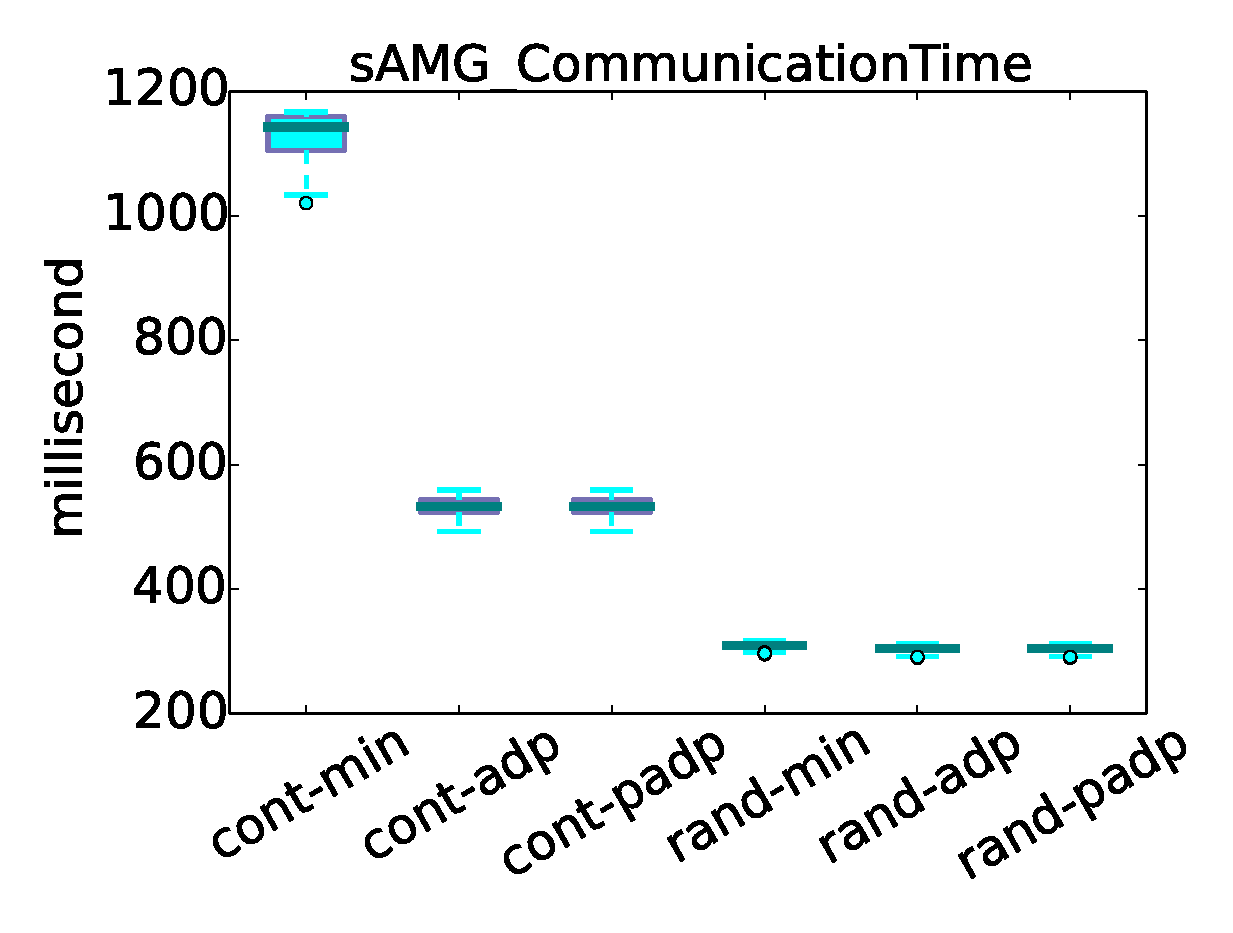
\includegraphics[height=1.5 in]{syn-wkld/amg10/commtime}
        \caption{sAMG}
        \label{fig:syn-samg-commtime}
    \end{subfigure}%
    \caption{Communication time distribution across application ranks in Workload~\Rmnum{2}. The ``bully", sAMG, benefits from random placement and adaptive routing, while the ``bullied", MultiGrid and CrystalRouter, suffer performance degradation.}
   \label{fig:syn-apps-commtime}
\end{figure*}



% explain the network status of sAMG, MG and CR
Once again, we look at the network-level system view to scrutinize the traffic through the routers serving each application. 
The routers serving sAMG have a high volume of traffic on both local and global channels when contiguous placement is in use, 
as shown in Figures~\ref{fig:syn-samg-lc-traffic} and \ref{fig:syn-samg-gc-traffic}.
As in previous results, the use of random placement alleviates the local congestion by uniformly distributing the traffic of sAMG over the network, getting more routers involved in serving sAMG.
In this case, a majority of those less busy routers are also serving MultiGrid and CrystalRouter.



%MultiGrid and CrystalRouter are the less communication-intensive applications in Workload~\Rmnum{2}.
% JJ - I shortened this
%When MultiGrid is running with contiguous placement, the serving routers have a comparatively small volume of traffic on their local and global channels, as shown in Figure~\ref{fig:syn-mg-lc-traffic} and \ref{fig:syn-mg-gc-traffic}. When coupled with (progressive) adaptive routing, more MultiGrid traffic traverses global channels, while more aggregate traffic is seen on the local channels due to the additional intermediate hops.
%When random placement is in use, the MPI ranks of MultiGrid are randomly distributed across the network and share routers with other applications. The routers serving MultiGrid have much more traffic on their local and global channels, as shown in Figures~\ref{fig:syn-mg-lc-traffic} and \ref{fig:syn-mg-gc-traffic}. The increased traffic comes largely from sAMG. \TODO{can shorten this}

MultiGrid in Workload~\Rmnum{2} appears most similar to AMG in Workload~\Rmnum{1} when considering resident channel behavior, as shown in Figures~\ref{fig:syn-mg-lc-traffic} and \ref{fig:syn-mg-gc-traffic}. There is a large gap in traffic volume between the contiguous and random placement approaches, due to other applications (sAMG in particular) utilizing the same links. CrystalRouter in Workload~\Rmnum{2} additionally experiences more load on its channels using random allocation configurations, as shown in Figure~\ref{fig:syn-cr-lc-traffic} and \ref{fig:syn-cr-lc-traffic}. However, the maximal load under random allocation is closer to that seen in contiguous allocations as compared to MultiGrid.

\begin{figure*}[t]
    \centering
    \begin{subfigure}[t]{0.32\textwidth}
        \centering
        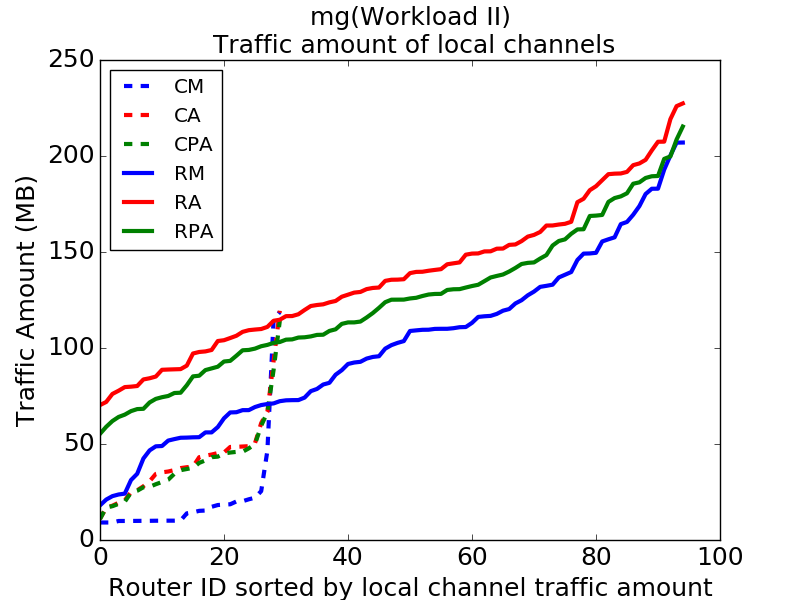
\includegraphics[height=1.5 in]{syn-wkld/mg/lc-traffic}
        \caption{MultiGrid Local Channel Traffic}
        \label{fig:syn-mg-lc-traffic}
    \end{subfigure}\hfill
    \begin{subfigure}[t]{0.32\textwidth}
        \centering
        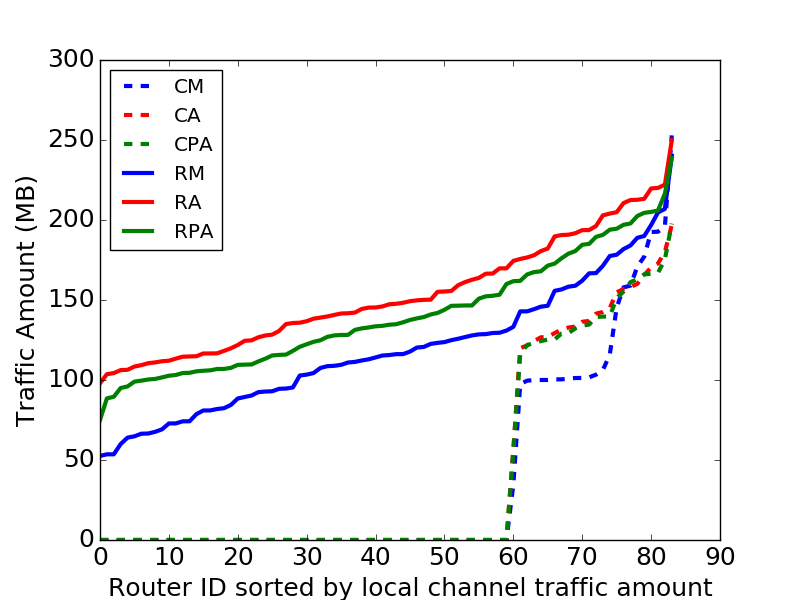
\includegraphics[height=1.5 in]{syn-wkld/cr/lc-traffic}
        \caption{CrystalRouter Local Channel Traffic}
        \label{fig:syn-cr-lc-traffic}
    \end{subfigure}\hfill
    \begin{subfigure}[t]{0.32\textwidth}
        \centering
        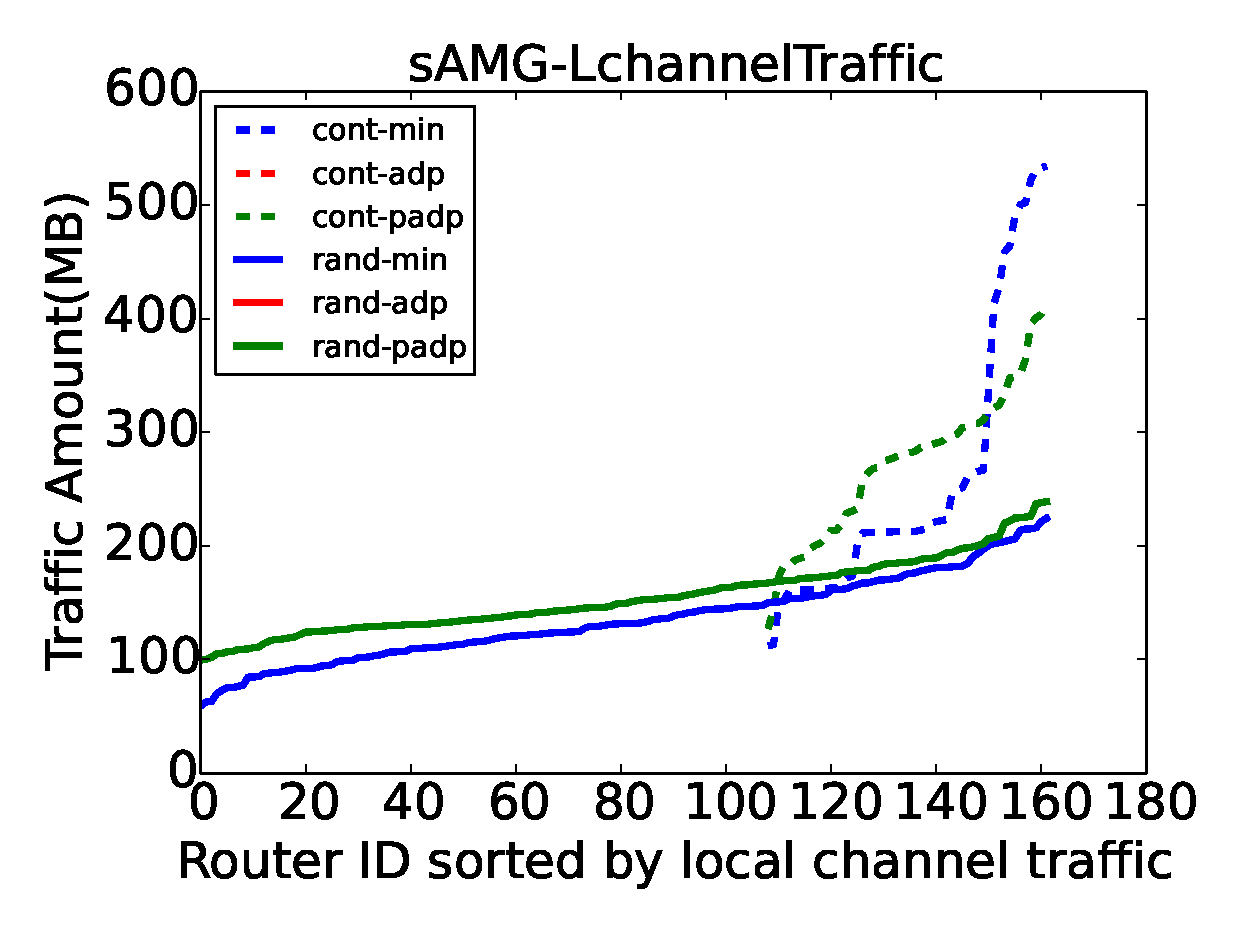
\includegraphics[height=1.5 in]{syn-wkld/amg10/lc-traffic}
        \caption{sAMG Local Channel Traffic}
        \label{fig:syn-samg-lc-traffic}
    \end{subfigure}\\
    \centering
    \begin{subfigure}[t]{0.32\textwidth}
        \centering
        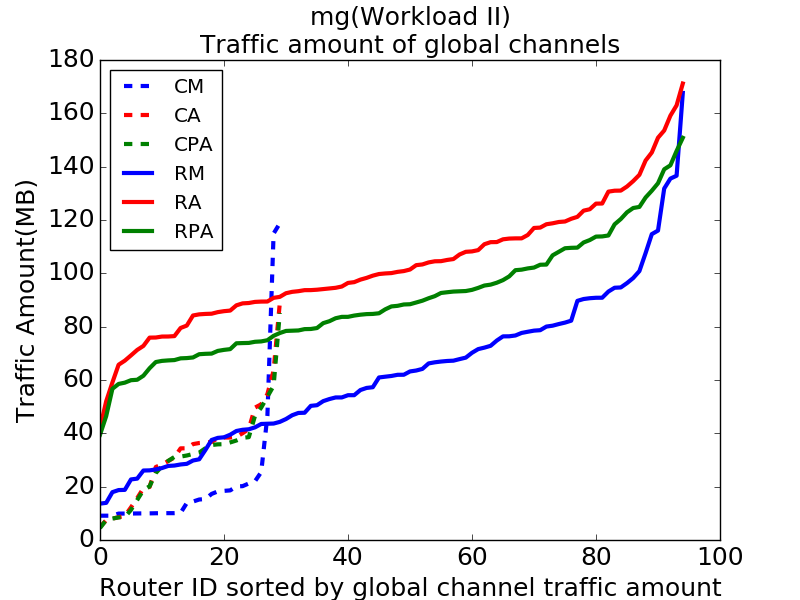
\includegraphics[height=1.5 in]{syn-wkld/mg/gc-traffic}
        \caption{MultiGrid Global Channel Traffic}
        \label{fig:syn-mg-gc-traffic}
    \end{subfigure}\hfill
    \begin{subfigure}[t]{0.32\textwidth}
        \centering
        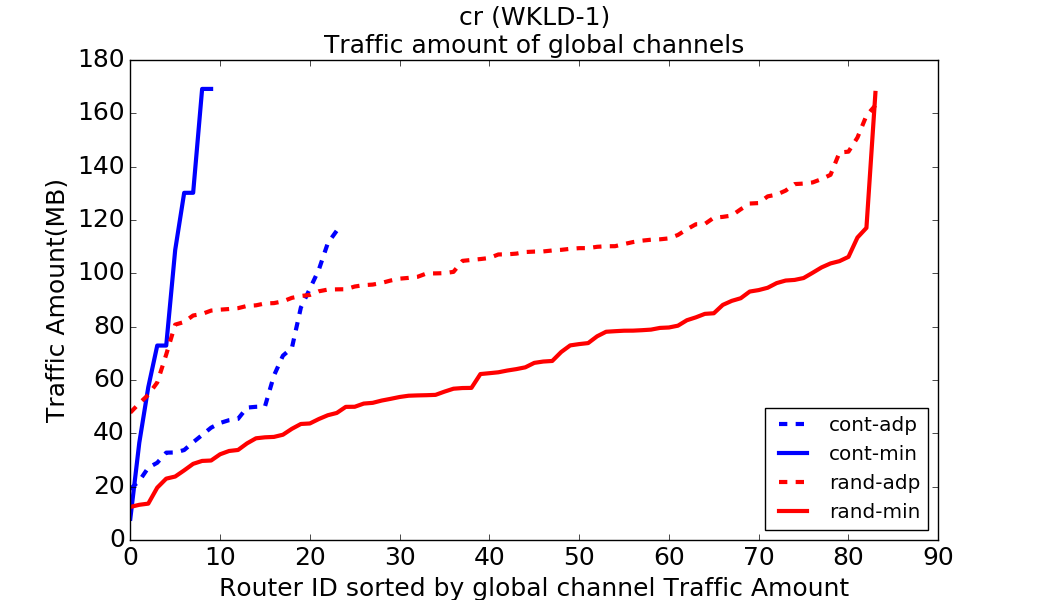
\includegraphics[height=1.5 in]{syn-wkld/cr/gc-traffic}
        \caption{CrystalRouter Global Channel Traffic}
        \label{fig:syn-cr-gc-traffic}
    \end{subfigure}\hfill
    \begin{subfigure}[t]{0.32\textwidth}
        \centering
        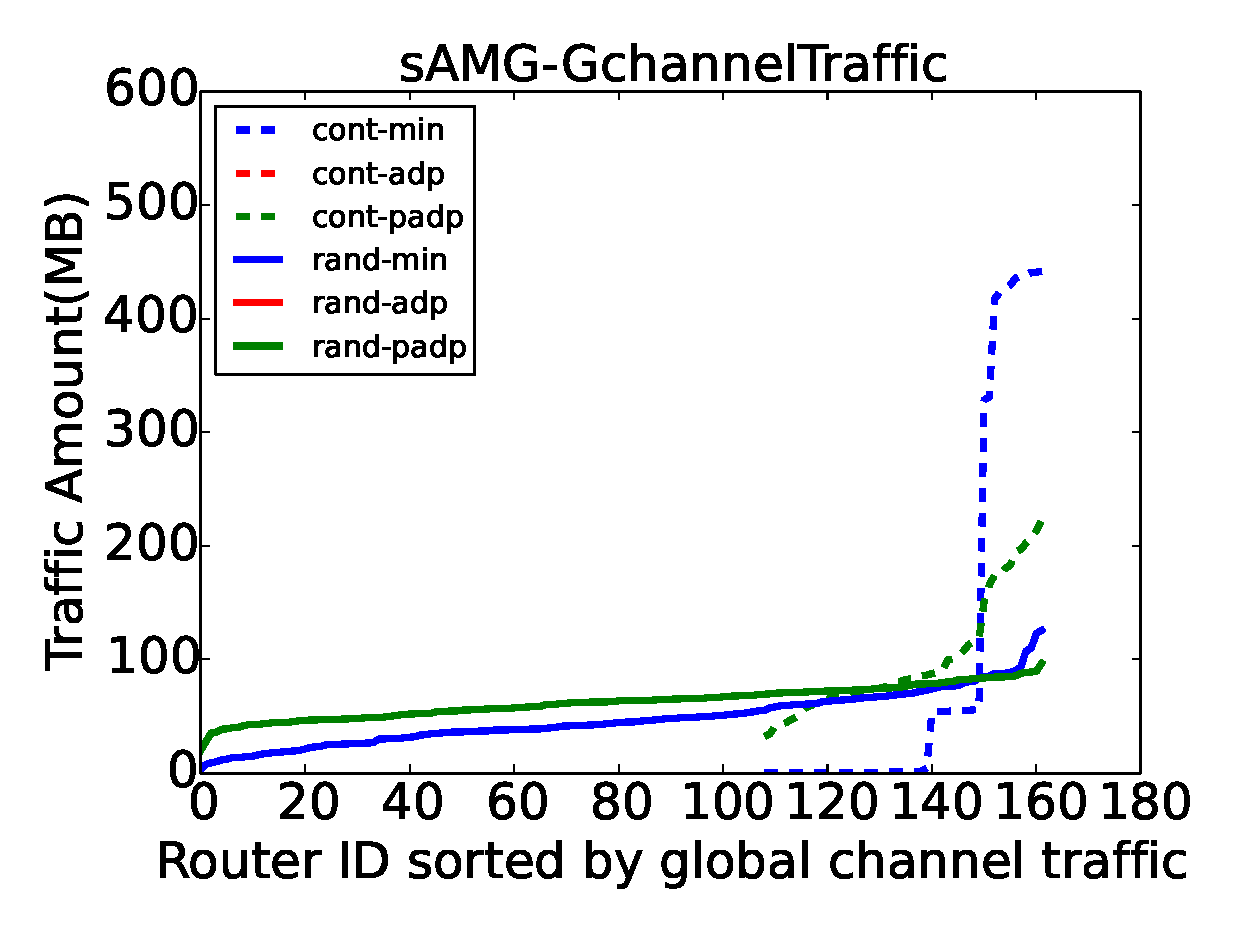
\includegraphics[height=1.5 in]{syn-wkld/amg10/gc-traffic}
        \caption{sAMG Global Channel Traffic}
        \label{fig:syn-samg-gc-traffic}
    \end{subfigure}
    \caption{Aggregate workload traffic for routers serving specific applications. More routers are involved in serving each application when random placement is in use, compared to contiguous placement.}
   \label{fig:syn-3app-gc-traffic}
\end{figure*}



\subsection{Observations}

\NOTE{rewrote this somewhat. The observations made were essentially the same
as the previous section}

Revisiting the observations in Section~\ref{sec:workload-1-observations}, we
find that those observations are held under this separate configuration.
System-level performance is still much improved in terms of load-balancing.
sAMG, being far and away the most communication-intensive application, benefits
greatly from random placement, whereas in Workload~\Rmnum{1} AMG was effectively
penalized for being less communication-intensive. CrystalRouter, being the
comparatively less communication-intensive application in Workload~\Rmnum{2},
experiences performance regressions in Workload~\Rmnum{2} under random and adaptive
policies.

Interestingly, in both Workload~\Rmnum{1} and \Rmnum{2}, MultiGrid experiences
a more subtle performance behavior than the significant swings in performance
seen in the other applications. These behaviors persisted across multiple runs
with different random seeds. Additionally, CrystalRouter in Workload~\Rmnum{2}
sees less drastic changes in maximal load, but still experiences performance
regressions. We are continuing to work towards understanding the root causes
and implications of this behavior, for which we expect application-specific
communication patterns to be an important factor. \TODO{Is this a reasonable
observation?}


\section{Hybrid Job Placement}
\label{sec: hybrid placement}

Based on our experiments with Workloads~\Rmnum{1} and \Rmnum{2}, the ``bully" behavior is
exhibited when the dragonfly network is configured with random placement and
(progressive) adaptive routing, and there is a large gap between the
communication intensity of applications running on the network.
As shown through our experimentation, contiguous placement policies give up too
much in terms of congestion and load balance, hence being an impractical solution. 
Further, running each job with a dedicated routing policy is unrealistic, 
since routing policy is part of system configuration which can not be changed
on the fly upon job submission. 
%and the policies of some jobs (adaptive) will still interfere with others.


As a natural extension of our observations, one question that arises is \emph{whether
we can combine the merits of random and contiguous placement policies in
which each application receives the performance benefits from system load
balancing while avoiding the ``bully'' behavior.} As an initial exploration of
the question, we set up a mock hybrid job placement policy, in which less
communication-intensive jobs receive contiguous allocations to avoid the
``bully" effect, while the communication-intensive jobs are allocated randomly
in order to distribute the communication load. For Workload~\Rmnum{1}, this
means AMG gets a contiguous allocation while MultiGrid and CrystalRouter get
random allocations. Note that we do not consider challenges inherent in
designing an allocation policy for production usage, such as backfilling,
reserving large contiguous sets of nodes, determining a metric for
communication intensity, etc., preferring a restricted-scope experiment
looking at the design space of dragonfly allocation policies in light of our experimental
observations.


%\subsection{Network Performance Analysis}
%
%Hybrid placement is also coupled with three routing policies, minimal, adaptive and progressive adaptive, denoted respectively as HM, HA and HPA. As presented in section~\ref{sec: workload-1 network analysis} and~\ref{sec: workload-2 network analysis}, random placement outperforms contiguous placement in terms of network performance, the analysis in this section only focuses on the comparison between hybrid and random placement policies. 
%
%\begin{table}[ht]
%\begin{center}
%\caption{Average time spent on communication by all MPI ranks when Workload I is running on dragonfly network under hybrid placement and random placement policies.} 
%\label{tab: hyb-placement-wkld-commtime}
%\begin{tabular}{l c c c c c c }
%\toprule % Top horizontal line
%\toprule
%&\multicolumn{6}{c}{Placement and Routing Configurations} \\
%\cmidrule(l){2-7}
%          & HM & HA & HPA & RM & RA & RPA \\ % Column names row
%\midrule % In-table horizontal line
%Time(ms)  &273 &255 &255 &255 &265 &264  \\ % Content row 1
%%\midrule
%%Workload II &1747 &1991 &1991 &1791 &2367 &1965 \\
%\midrule % In-table horizontal line
%\bottomrule % Bottom horizontal line
%\end{tabular}
%\end{center}
%\end{table}
%
%Due to page limit, we only present the average communication time spent by Workload~\Rmnum{1} for the evaluation of the network performance.
%\footnote{The analysis about network traffic and saturated time are omitted in this section due to page limit.}
%As shown in Table~\ref{tab: hyb-placement-wkld-commtime}, 
%hybrid placement coupled with (progressive) adaptive routing (HA, HPA) can guarantee the same performance as random placement coupled with minimal routing (RM), thus the average workload communication time stays unchanged. 
%When hybrid placement coupled with minimal routing (HM) is in use, 
%the network performance declines  as indicated by the increasing average communication time. 
%The consecutive groups assigned to AMG results in the diminishing of network resource shared by MultiGrid and CrystalRouter, 
%causing unbalanced utilization over the network.  



%\subsection{Individual Application Analysis}

\begin{figure*}[t!]
    \centering
    \begin{subfigure}[t]{0.32\textwidth}
        \centering
        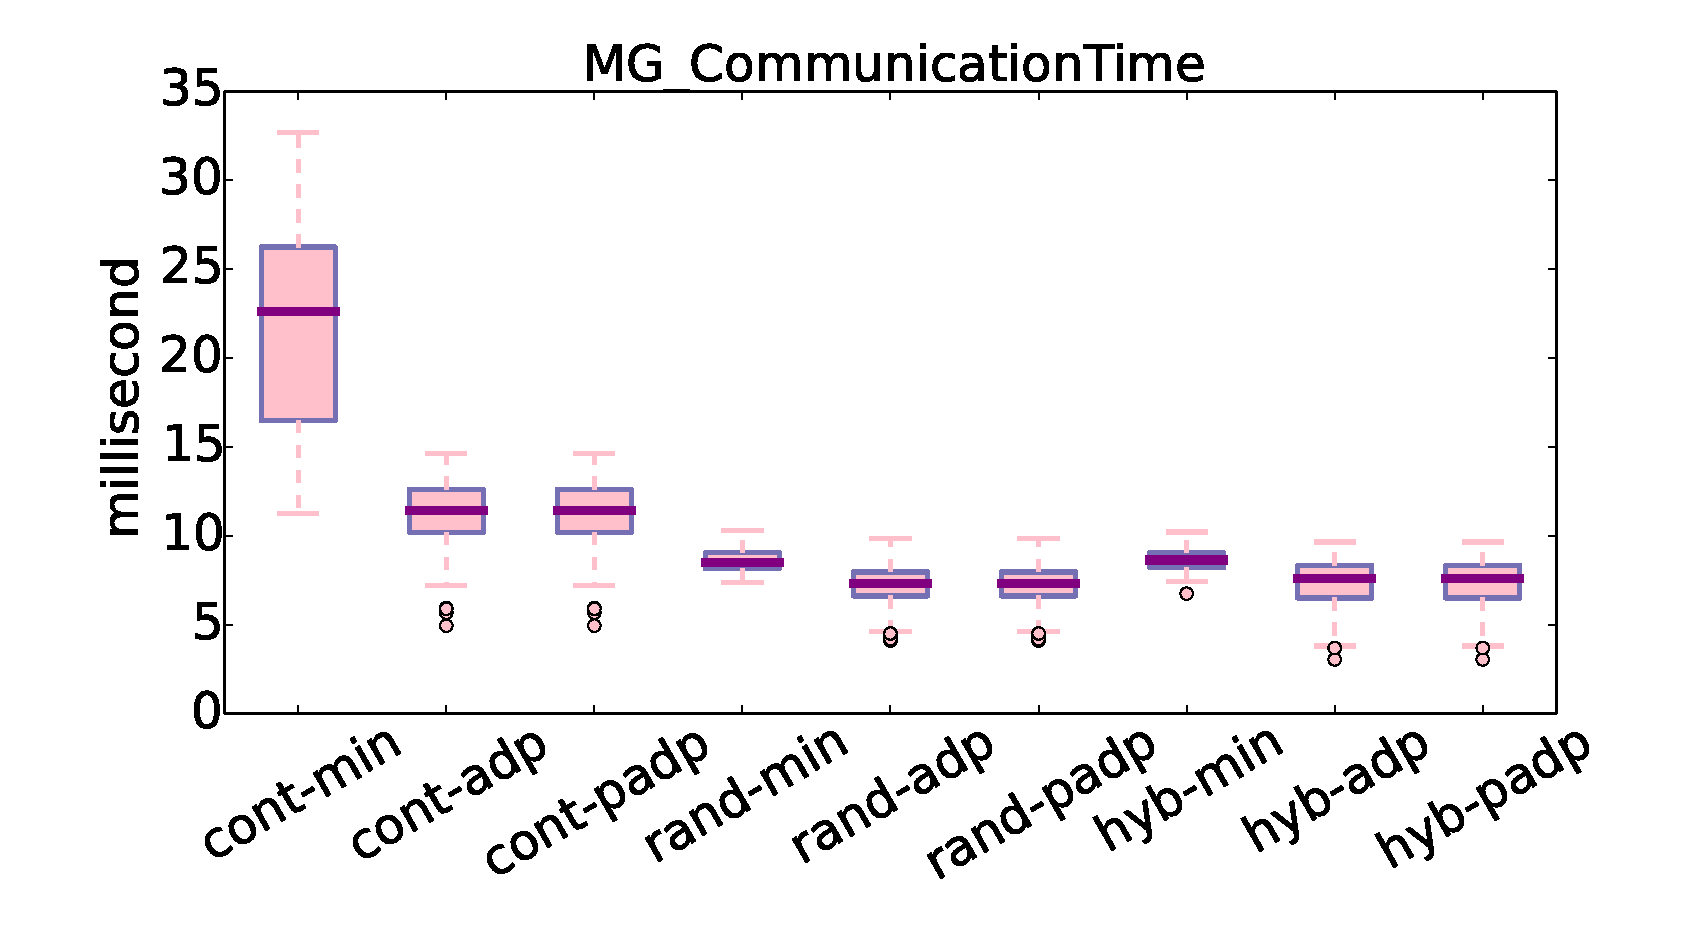
\includegraphics[height=1.3 in]{hyb-plcmt/mg/commtime}
        \caption{MultiGrid Communication Time}
        \label{fig:hyb-plcmt-mg-commtime}
    \end{subfigure}\hfill
    \begin{subfigure}[t]{0.32\textwidth}
        \centering
        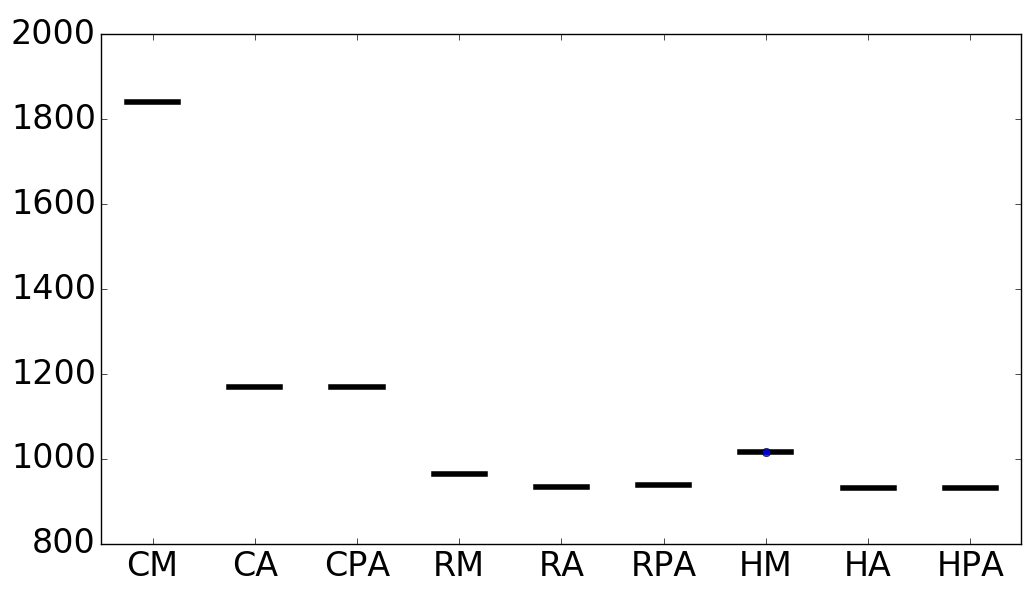
\includegraphics[height=1.3 in]{hyb-plcmt/cr/commtime}
        \caption{CrystalRouter Communication Time}
        \label{fig:hyb-plcmt-cr-commtime}
    \end{subfigure}\hfill
    \begin{subfigure}[t]{0.32\textwidth}
        \centering
        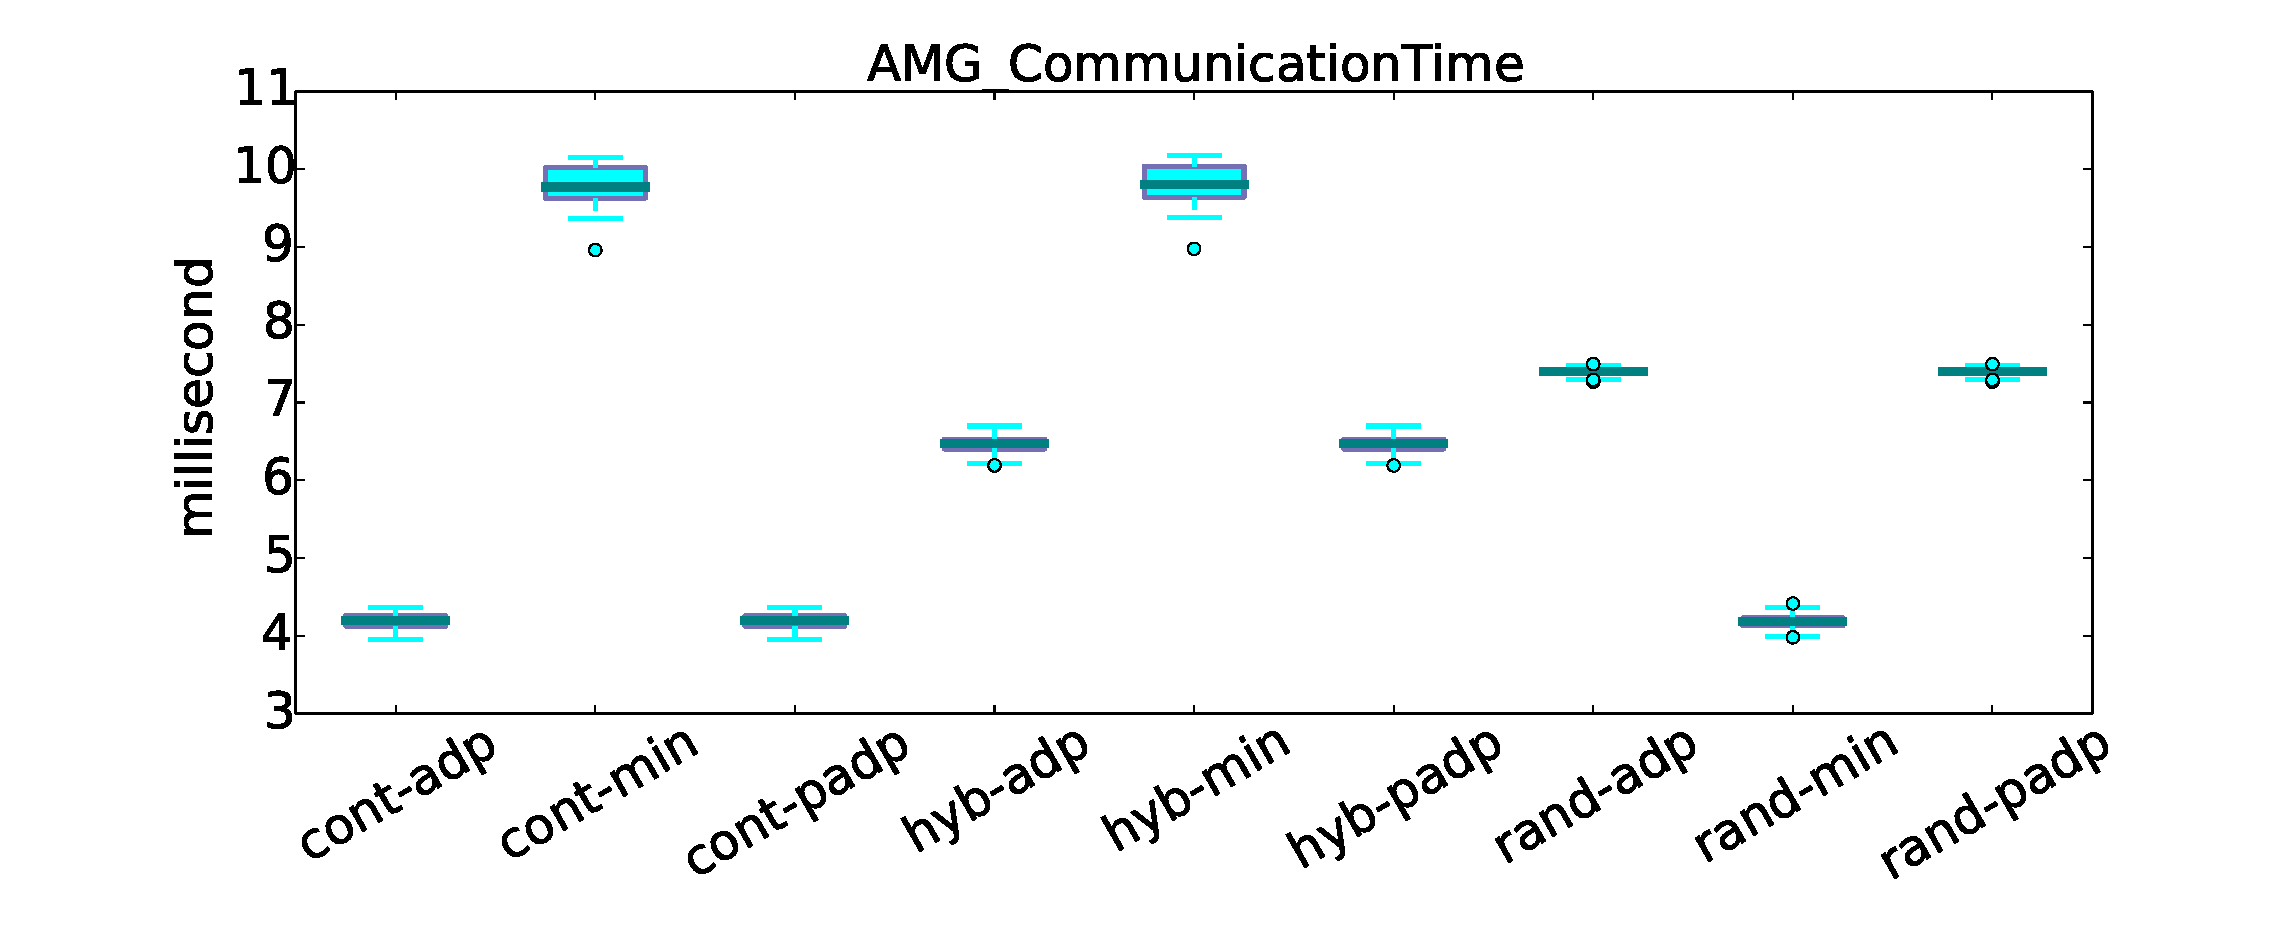
\includegraphics[height=1.3 in]{hyb-plcmt/amg/commtime}
        \caption{AMG Communication Time}
        \label{fig:hyb-plcmt-amg-commtime}
    \end{subfigure}
   \caption{Application communication time. Workload~\Rmnum{1} is running with all placement and routing configurations. Methods prefixed with ``H'' represent the hybrid allocation approach.}
   \label{fig:hyb-plcmt-apps-commtime}
\end{figure*}

For the purpose of brevity, we only present the
communication time distribution of each application under all placement and routing configurations, including the hybrid placement method. These results are presented in Figure~\ref{fig:hyb-plcmt-apps-commtime}. 
As shown in Figure~\ref{fig:hyb-plcmt-mg-commtime} and~\ref{fig:hyb-plcmt-cr-commtime},
MultiGrid and CrystalRouter exhibit similar performance in both hybrid and random placement, as nodes are being placed randomly in each case.
While the performance of AMG under hybrid placement, shown in Figure~\ref{fig:hyb-plcmt-amg-commtime}, still appears to exhibit significant communication interference on account of the other applications as opposed to the best contiguous placement policies, the effects are reduced compared to a random-adaptive policy. We believe this to be a result of more AMG-specific traffic occupying a smaller set of routers/groups, both reducing the probability of traffic entering them through adaptive routing and increasing the relative proportion of link utilization by AMG. Of course, this comes with the costs associated with contiguous allocation, in which AMG's traffic is less likely to load balance across multiple dragonfly groups.

%\TODO{How's this? Awesome}
These initial experiments demonstrate some degree of benefit derived from using a hybrid approach, helping to alleviate the ``bully'' effect while retaining the performance of communication-intensive applications. However, the behavior is still not ideal in this case -- AMG's communications still experience performance degradation versus the contiguous configurations. Hence, more work in this area is needed to fully understand the intricate relationships between job scheduling and system/application communication behavior to achieve optimal network utilization and application performance in high-radix networks.


\section{Related Work}
\label{sec:related work}

The impact of job placement on both systems and applications has been the subject of many studies~\cite{dskinner,abhinav-sc13,jose-ipdps15}. We focus on the HPC-centric studies here. Skinner et al.\ identified significant performance variability due to network contention.~\cite{dskinner}. They found that performance variability is inevitable on either torus or fat-tree networks when network sharing among concurrently running applications is allowed.
%\TODO{what kind of system?}. 
Bhatele et al.\ studied the performance variability of a specific application, p3FD, running on different HPC production systems with torus network topologies \cite{abhinav-sc13}. They obtained performance consistency in their application when network resources were allocated compactly and exclusively and wide variability otherwise. Jokanovic et al. studied the impact of job placement to the workload and claimed that the key to reduce performance variability is to avoid network sharing~\cite{jose-ipdps15}. 

Recently, several researchers have investigated job placement and routing algorithms on dragonfly networks. Bogdan et al.\ proposed a communication-matrix-based analytic modeling framework for mapping application workloads onto network topologies~\cite{hoefler-hpdc14}. They found that, in the context of dragonfly networks, optimizing for throughput and not workload completion time is often misleading and the notion of system balance cited as a dragonfly design parameter is not always directly applicable to all workloads.
%\TODO{very brief blurb of what they did or what they found}. 
Jain et al. conducted a comprehensive analysis of various job placement and routing policies with regard to network link throughput on dragonfly network~\cite{jain-sc14}. Their work is based on an analytical model and synthetic workload. Bhatele et al. used coarse-grain simulation to study the performance of synthetic workloads under the different task mapping and routing policies on two-level direct networks~\cite{bhatele-sc11}. Mubarak et al.\ focused on  the modeling of large-scale dragonfly networks with parallel event driven simulation. The dragonfly network model for million-node configurations presented in their work strongly scales when going from 1,024 to 65,536 MPI tasks on IBM Blue Gene/P and IBM Blue Gene/Q systems~\cite{codes-dragonfly}. The dragonfly model used in this paper is from their work. 
%\TODO{mention Misbah's dragonfly work, for which our work is based on}.

Our work complements the literature in the following ways. First, our simulations are driven by real application traces intended to be representative of production-scale application patterns. Second, we holistically examine behavior at both the overall system level as well as the application level, though we do not consider communication-pattern specific application mappings as Bogdan et al.\ did. Third, with the CODES simulation toolkit and related network models~\cite{codes, codes-dragonfly},  
%\TODO{cite codes, Misbah's dragonfly work}, 
we are able to simulate and examine system and application behavior at a very fine grain, collecting data at the dragonfly link level with packet-level fidelity. We believe these differences allowed us to uncover the ``bullying'' behavior, which to our knowledge is unreported in the literature. However, in a sense, Bogdan et al.'s work suggests these types of behaviors as possibilities deriving from the balance-first design rationale for the dragonfly.


\section{Conclusion}
\label{sec:conclusion}

In this paper, we have conducted extensive study about application's behavior when running on dragonfly network with different job placement and routing configurations. We resorted to CODES, a high-fidelity HPC network simulation tool, and used three parallel scientific applications traces collected from production system to analyze the applications' behavior on network level. We found that when applications are running concurrently, although random placement can uniformly distribute the workload traffic over the network to reach load balance and hot-spots free for the network, the performance of certain job would be impaired. We identify this phenomenon as ``bully" between concurrently running jobs, and the victim always being the less communication-intensive one. On the other hand, the contiguous placement tend to cause local congestion, however when coupled with adaptive routing, it can guarantee the performance of ``bullee" application by limiting the network sharing from concurrently running peers. 

Due the presence of this ``bully", we propose to use hybrid placement policy for workload running on systems with dragonfly networks. In hybrid placement policy, the less intensive applications get contiguous allocations, and the intensive ones get random allocations. We believe the findings presented in this paper can illuminate a path to more efficient workload manager for future systems with dragonfly network.




% conference papers do not normally have an appendix



% use section* for acknowledgment
\ifCLASSOPTIONcompsoc
  % The Computer Society usually uses the plural form
  \section*{Acknowledgments}
\else
  % regular IEEE prefers the singular form
%   \section*{Acknowledgment}
\fi


The work at Illinois Institute of Technology is supported in part by U.S. National Science Foundation grants CNS-1320125 and CCF-1422009. This work is also supported by the U.S. Department of Energy, Office of Science, Advanced Scientific Computing Research, under Contract DE-AC02-06CH11357.


% trigger a \newpage just before the given reference
% number - used to balance the columns on the last page
% adjust value as needed - may need to be readjusted if
% the document is modified later
%\IEEEtriggeratref{4}


\bibliographystyle{IEEEtran}
\bibliography{IEEEabrv,reference}


\vspace{1\baselineskip}
 
\begin{framed}
 The submitted manuscript has been created by UChicago Argonne, LLC, Operator of Argonne National Laboratory ("Argonne").  Argonne, a U.S. Department of Energy Office of Science laboratory, is operated under Contract No. DE-AC02-06CH11357.  The U.S. Government retains for itself, and others acting on its behalf, a paid-up nonexclusive, irrevocable worldwide license in said article to reproduce, prepare derivative works, distribute copies to the public, and perform publicly and display publicly, by or on behalf of the Government.
\end{framed}


\end{document}


